\mfpicnumber{1}

\opengraphsfile{FunctionsandtheirRepresentations}

\setcounter{footnote}{0}

\label{FunctionsandtheirRepresentations}


\subsection{Functions as Mappings}

Mathematics can be thought of as the study of patterns.   In most disciplines, Mathematics is used as a language to express, or codify, relationships between quantities  - both algebraically and geometrically - with the ultimate goal of solving real-world problems.   The fact that the same algebraic equation which models the growth of bacteria in a petri dish is also used to compute the account balance of a savings account or the potency of radioactive material used in medical treatments speaks to the universal nature of Mathematics.   Indeed, Mathematics is more than just about solving a specific problem in a specific situation, it's about abstracting problems and creating universal tools which can be used by a variety of scientists and engineers to solve a variety of problems.  

\medskip

This power of abstraction has a tendency to create a language that is initially intimidating to students.  Mathematical definitions are precise and adherence to that precision is often a source of confusion and frustration.  It doesn't help matters that more often than not very common words are used in Mathematics with slightly different definitions than is commonly expected.  The first `universal tool' we wish to highlight - the concept of a `function' - is a perfect example of this phenomenon in that we redefine a word that already has multiple meanings in English.  

\medskip

\colorbox{ResultColor}{\bbm

\begin{defn}[Function]

\label{functiondefn}

Given two sets\footnote{Please refer to Section \ref{AppSetTheory} for a review of this terminology.} $A$ and $B$, a  \index{function ! definition} \textbf{function} from $A$ to $B$ is a process by which each element of $A$ is matched with (or `mapped to')  one and only one element of $B$.   

\end{defn}

\ebm}

\medskip

The grammar here `\textit{from} $A$ \textit{to} $B\,$'  is important.  Thinking of a function as a process, we can view the elements of the set $A$ as our starting materials, or \textit{inputs} to the process.  The function  processes these inputs according to some specified rule and the result is a set of  \textit{outputs}  - elements of the set $B$. In terms of inputs and outputs, Definition \ref{functiondefn}  says that a function is a process in which each \textit{input} is matched to one and only one \textit{output}.

\medskip

For example, let's take a look at some of the pets in the Stitz household.  Taylor's pets include White Paw and Cooper (both cats), Bingo (a lizard) and Kennie (a turtle).  Let $N$ be the set of pet names: $N = \{ \text{White Paw, Cooper, Bingo, Kennie} \}$, and let $T$ be the set of pet types:  $T = \{ \text{cat, lizard, turtle} \}$.   Let $f$ be the process that takes each pet's name as the input and returns that pet's type as the output. Let $g$ be the reverse of $f$:  that is, $g$ takes each pet type as the input and returns the names of the pets of that type as the output.   Note that both $f$ and $g$ are codifying the \textit{same} given information about Taylor's pets,  but one of them is a function and the other is not.  

\medskip

To help identify which process $f$ or $g$ is a function and  why the other is not, we create  \index{diagram ! mapping} \textbf{mapping diagrams} for $f$ and $g$ below.  In each case, we organize the inputs in a column on the left and the outputs on a column on the right.  We draw an arrow connecting each input to its corresponding output(s).  Note that the arrows communicate the grammatical bias: the arrow originates at the input and points to the output.

\medskip

\begin{center}

\begin{tabular}{cc}
\begin{mfpic}[19]{-5}{5}{2}{6}
\tlabel[cc](-4.25,6){$N$ (inputs)}
\tlabel[cc](-4.25,5){White Paw}
\tlabel[cc](-4.25,4){Cooper}
\tlabel[cc](-4.25,3){Bingo}
\tlabel[cc](-4.25,2){Kennie}
\tlabel[cc](0,6){$f$}
\tlabel[cc](3.5,5){cat}
\tlabel[cc](3.5,4){lizard}
\tlabel[cc](3.5,3){turtle}
\tlabel[cc](3.5,6){$T$ (outputs)}


\arrow[l 5pt] \polyline{(-2.5, 5), (2.5, 5)}
\arrow[l 5pt] \polyline{(-2.5, 4), (2.5, 5)}
\arrow[l 5pt] \polyline{(-2.5, 3), (2.5, 4)}
\arrow[l 5pt] \polyline{(-2.5, 2), (2.5, 3)}

\end{mfpic}

&
\begin{mfpic}[19]{-5}{5}{2}{6}
\tlabel[cc](-3.5,6){$T$ (inputs)}
\tlabel[cc](-3.5,5){cat}
\tlabel[cc](-3.5,4){lizard}
\tlabel[cc](-3.5,3){turtle}
\tlabel[cc](0,6){$g$}
\tlabel[cc](3.75,6){$N$ (outputs)}
\tlabel[cc](3.75,5){White Paw}
\tlabel[cc](3.75,4){Cooper}
\tlabel[cc](3.75,3){Bingo}
\tlabel[cc](3.75,2){Kennie}
\arrow[l 5pt] \polyline{(-2.5, 5), (2.5, 5)}
\arrow[l 5pt] \polyline{(-2.5, 5), (2.5, 4)}
\arrow[l 5pt] \polyline{(-2.5, 4), (2.5, 3)}
\arrow[l 5pt] \polyline{(-2.5, 3), (2.5, 2)}
\end{mfpic}   \\

\end{tabular}

\end{center}

The process $f$ is a function since $f$ matches each of its inputs (each pet name) to just one output (the pet's type).   The fact that different inputs (White Paw and Cooper) are matched to the same output (cat) is fine.   On the other hand, $g$ matches the input `cat' to the two different outputs  `White Paw' and `Cooper', so $g$ is not a function.    Functions are favored in mathematical circles because they are processes which produce only one answer (output) for any given query (input).  In this scenario, for instance, there is only one answer to the question: `What type of pet is White Paw?' but there is more than one answer to the question `Which of Taylor's pets are cats?'  

\medskip

As you might expect, with functions being such an important concept in Mathematics, we need to build a vocabulary to assist us when discussing them.  To that end, we have the following definitions.\footnote{Please refer to Section \ref{AppSetTheory} for a review of the terminology used in these definitions.}

\medskip

\colorbox{ResultColor}{\bbm

\begin{defn}

\label{domainrangedefns}

Suppose $f$ is a function from $A$ to $B$.

\begin{itemize}

\item If $a \in A$, we write $f(a)$ (read `$f$ of $a\, $') to denote the unique element of $B$ to which $f$ matches $a$.  

That is, if we view `$a\,$' as the input to $f$, then `$f(a)$' is the output from $f$.

\item  The set $A$ is called the \index{domain ! definition} \textbf{domain}.  

Said differently, the domain of a function is the set of inputs to the function.

\item  The set $\{ f(a) \, | \, a \in A \}$ is called the  \index{range ! definition}  \textbf{range} of $f$. 

Said differently, the range of a function is the set of outputs from the function.

\end{itemize}


\end{defn}

\ebm}

Some remarks about Definition \ref{domainrangedefns} are in order.  First, and most importantly, the notation `$f(a)$' in Definition \ref{domainrangedefns}  introduces yet another mathematical use for parentheses.  Parentheses are used in some cases as grouping symbols, to represent ordered pairs, and to delineate intervals of real numbers.  More often than not, the use of parentheses in expressions like `$f(a)$' is confused with multiplication.   As always, paying attention to the context is key.  If $f$ is a function and `$a\,$' is in the domain of $f$, then `$f(a)$'  is the output from $f$ when you input $a$.  The diagram below provides a nice generic picture to keep in mind when thinking of a function as a mapping process with input `$a\,$' and output `$f(a)$'.

\begin{center}

%\scriptsize

\begin{mfpic}[10]{-10}{10}{-10}{10}
\tlabel[cc](0,6){$f$}
\tlabel[cc](-9,-1){$a$}
\tlabel[cc](-9,-3){input}
\tlabel[cc](7,-1){$ f(a)$}
\tlabel[cc](7,-3){output}
\point[2pt]{(-9,0), (7,0)} 
\sclosed \curve{(-6,7), (-12,0), (-6,-9), (-7,0)}
\tlabel[cc](-9,-10){$A$}
\sclosed \curve{(6,7), (11,0), (5,-8)}
\tlabel[cc](7,-10){$B$}
\penwd{0.75pt}
\arrow \curve{(-8.75,0.25), (0,5), (6.75,0.25)}
\end{mfpic}

\end{center}

%\normalsize

In the preceding pet example, the symbol $f(\text{Bingo})$, read `$f$ of Bingo', is asking what type of pet Bingo is, so $f(\text{Bingo}) = \text{lizard}$.  The fact that $f$ is a function means $f(\text{Bingo})$ is unambiguous because $f$ matches the name `Bingo' to only one pet type, namely `lizard'. In contrast, if we tried to use the notation `$g(\text{cat})$' to indicate what pet name $g$ matched to `cat', we have \textit{two} possibilities, White Paw and Cooper, with no way to determine which one (or both) is indicated.  

\medskip

Continuing to apply Definition \ref{domainrangedefns} to our pet example, we find that the domain of the function $f$ is $N$, the set of pet names.  Finding the range takes a little more work, mostly because it's easy to be caught off guard by the notation used in the definition of `range'.  The description of the range as `$\{ f(a) \, | \, a \in A \}$' is an example of `set-builder' notation.  In English,  `$\{ f(a) \, | \, a \in A \}$'  reads as `the set of $f(a)$ such that $a$ is in $A$'.  In other words, the range consists of all of the outputs from $f$ - all of the $f(a)$ values - as $a$ varies through each of the elements in the domain $A$.   Note that while every element of the set $A$ is, by definition, an element of the domain of $f$, not every element of the set $B$ is necessarily part of the range of $f$.\footnote{For purposes of completeness, the set $B$ is called the \index{codomain ! definition} \textbf{codomain} of $f$.  For us, the concepts of domain and range suffice since our codomain will most always be the set of real numbers, $\mathbb{R}$.}

\medskip

In our pet example, we can obtain the range of $f$  by looking at the mapping diagram or by constructing the set $\{ f(\text{White Paw}), f(\text{Cooper}), f(\text{Bingo}), f(\text{Kennie}) \}$ which lists all of the outputs from $f$ as we run through all of the inputs to $f$.   Keep in mind that we list each element of a set only once so the range of $f$ is:\footnote{If instead of mapping $N$ into $T$, we could have mapped $N$ into $U=\{ \text{cat}, \text{lizard}, \text{turtle}, \text{dog}\}$ in which case the range of $f$ would not have been the entire codomain $U$.}  \[ \{ f(\text{White Paw}), f(\text{Cooper}), f(\text{Bingo}), f(\text{Kennie}) \} = \{ \text{cat}, \text{lizard}, \text{turtle} \} = T.\] 


If we let $n$ denote a generic element of $N$ then $f(n)$ is some element $t$ in $T$, so we write $t = f(n)$.  In this equation, $n$ is called the \index{variable ! independent}\textbf{independent variable} and $t$ is called the  \index{variable ! dependent}\textbf{dependent variable}.\footnote{These adjectives stem from the fact that the value of $t$ \textit{depends} entirely on our (independent) choice of $n$.}    Moreover, we say `$t$ is a function of $n\,$',  or, more specifically, `the type of pet is a function of the pet name'  meaning that every pet name $n$ corresponds to one, and only one, pet type $t$.   Even though $f$ and $t$ are different things,\footnote{Specifically, $f$ is a function so it requires and domain, a range and a rule of assignment whereas $t$ is simply the output from $f$.} it is very common for the  function and its outputs to become more-or-less synonymous, even in what are otherwise precise mathematical definitions.\footnote{In fact, it is not uncommon to see the name of the function as the same as the dependent variable. For example, writing `$y = y(x)$'  would be a way to communicate the idea that `$y$ is a function of $x$'.}  We will endeavor to point out such ambiguities as we move through the text.

\medskip

While the concept of a function is very general in scope, we will be focusing primarily on functions of real numbers because most disciplines use real numbers to quantify data.  Our next example explores a function defined using a table of numerical values.

\begin{ex} \label{timetempex1}   Suppose Skippy records the outdoor temperature every two hours starting at 6 a.m. and ending at 6 p.m. and summarizes the data in the table below:


\[\begin{array}{|c||c|}  \hline

  \text{time (hours after 6 a.m.)} &  \text{outdoor temperature} \\
	                               & \text{in degrees Fahrenheit} \\ \hline
 0 & 64  \\  \hline
 2 & 67  \\  \hline
 4 &  75  \\  \hline
 6 &  80 \\  \hline
 8 & 83  \\  \hline
 10 &  83 \\  \hline
 12 & 82  \\  \hline

\end{array}\]

\begin{enumerate}

\item  Explain why the recorded outdoor temperature is a function of the corresponding time. 

\item  Is time a function of the outdoor temperature?  Explain.

\item Let $f$ be the function which matches time to the corresponding recorded outdoor temperature.

\begin{enumerate}

\item  Find and interpret the following:

\begin{multicols}{5}

\begin{itemize}

\item  $f(2)$

\item  $f(4)$

\item  $f(2+4)$

\item  $f(2) + f(4)$

\item  $f(2) + 4$

\end{itemize}

\end{multicols}

\item  Solve and interpret $f(t) = 83$. 

\item  State the range of $f$.  What is lowest recorded temperature of the day?  The highest?  

\end{enumerate}

\end{enumerate}

%\pagebreak

{\bf Solution.}

\begin{enumerate}

\item  The outdoor temperature is a function of time because each time value is associated with only one recorded temperature.

\item  Time is not a function of the outdoor temperature because there are instances when different times are associated with a given temperature.  For example, the temperature $83$ corresponds to both of the times $8$ and $10$.

\item 

\begin{enumerate}

\item 

\begin{itemize}

\item To find $f(2)$, we look in the table to find the recorded outdoor temperature that corresponds to when the time is $2$.  We get $f(2) =  67$ which means that 2 hours after 6 a.m. (i.e., at 8 a.m.), the temperature is $67^{\circ}$F.

\item   Per the table, $f(4) = 75$, so the recorded outdoor temperature at 10 a.m. (4 hours after 6 a.m.) is $75^{\circ}$F.

\item   From the table, we find $f(2+4) = f(6) = 80$, which means that at noon (6 hours after 6 a.m.), the recorded outdoor temperature is $80^{\circ}$F.  

\item  Using results from above we see that  $f(2) + f(4) =  67 + 75 = 142$.  When adding $f(2) + f(4)$, we are adding the recorded outdoor temperatures at 8 a.m. (2 hours after 6 a.m.) and 10 a.m. (4 hours after 6 AM), respectively,  to get $142^{\circ}$F.  

\item We compute $f(2) + 4 = 67 + 4 = 71$.  Here, we are adding $4^{\circ}$F to the outdoor temperature recorded at 8 a.m..

\end{itemize}

\item  Solving $f(t) = 83$ means finding all of the input (time) values $t$  which produce an output value of $83$.  From the data, we see that the temperature is $83$ when the time is $8$ or $10$, so the solution to $f(t) = 83$ is $t = 8$ or $t = 10$.  This means the outdoor temperature is $83^{\circ}$F at 2 p.m. (8 hours after 6 a.m.) and at 4 p.m. (10 hours after 6 a.m.).

\item  The range of $f$ is the set of all of the outputs from $f$, or in this case, the outside recorded temperatures.  Based on the data, we get $\{ 64, 67, 75, 80, 82, 83\}$.  (Here again, we list elements of a set only once.)  The lowest recorded temperature of the day is  $64^{\circ}$F and the highest recorded temperature of the day is  $83^{\circ}$F. \qed

\end{enumerate}

\end{enumerate}

\end{ex}

A few remarks about Example \ref{timetempex1} are in order.  First, note that $f(2+4)$, $f(2)+f(4)$ and $f(2)+4$ all work out to be numerically different, and more importantly, all represent different things.\footnote{You may be wondering why one would ever compute these quantities.  Rest assured that we will use expressions like these in examples throughout the text.  For now, it suffices just to know that they are different.}  One of the common mistakes students make is to misinterpret expressions like these, so it's important to pay close attention to the syntax here.

\medskip

Next,  when solving $f(t) = 83$, the variable `$t\,$' is being used as a convenient `dummy' variable or placeholder in the sense that solving $f(t) = 83$ produces the same solutions as solving $f(x) = 83$, $f(w) = 83$,  or even $f(?) = 83$.  All of these equations are asking for the same thing:  what inputs to $f$ produce an output of $83$.  The choice of the letter `$t\,$' here makes sense since the inputs are {\bf t}ime values.  Throughout the text, we will endeavor to use meaningful labels when working in applied situations, but the fact remains that the choice of letters (or symbols) is completely arbitrary. 

\medskip

Finally, given that the range in this example was a finite set of real numbers, we could find the smallest and largest elements of it.  Here, they correspond to the coolest and warmest temperatures of the day, respectively, but the meaning would change if the function related different quantities.  In many applications involving functions, the end goal is to find the minimum or maximum values of the outputs of those functions (called\index{optimization}\index{function ! optimization} \textbf{optimizing} the function) so for that reason, we have the following definition.  

\medskip

\colorbox{ResultColor}{\bbm

\begin{defn}

\label{absmaxmindefn}

Suppose $f$ is a function whose range is a set of real numbers containing $m$ and $M$.

\begin{itemize}

\item  The value $m$ is called the \textbf{minimum}\footnote{also called `absolute' or `global' minimum} of $f$ if $m \leq f(x)$ for all $x$ in the domain of $f$. \index{minimum ! formal definition of}

That is, the minimum of $f$ is the smallest output from $f$, if it exists.

\item  The value $M$ is called the \textbf{maximum}\footnote{also called `absolute' or `global' maximum}  of $f$ if $f(x) \leq M$ for all $x$ in the domain of $f$. \index{maximum ! formal definition of}

That is, the maximum of $f$ is the largest output from $f$, if it exists.

\item  Taken together, the values $m$ and $M$ (if they exist) are called the \textbf{extrema}\footnote{also called the `absolute' or `global' extrema or the `extreme values'} of $f$.

\end{itemize}

\end{defn}

\ebm}

\medskip

Definition \ref{absmaxmindefn} is an example where the name of the function, $f$, is being used almost synonymously with its outputs in that when we speak of `the minimum and maximum of the \textit{function} $f\,$' we are really talking about the minimum and maximum values of the \textit{outputs} $f(x)$ as $x$ varies through the domain of $f$.  Thus we say that the \index{function ! (absolute) maximum}\index{maximum ! intuitive definition of} maximum of $f$ is $83$ and the \index{function ! (absolute, global) minimum}\index{minimum ! intuitive definition of} minimum of $f$ is $64$ when referring to the highest and lowest recorded temperatures in the previous example.  

\subsection{Algebraic Representations of Functions}  

By focusing our attention to functions that involve real numbers, we gain access to all of the structures and tools from prior courses in Algebra.  In this subsection, we discuss how to represent functions algebraically using formulas and begin with the following example.

\begin{ex} \label{funcnotatex1} $~$

\begin{enumerate}

\item  Let $f$ be the function which takes a real number and performs the following sequence of operations:

\begin{itemize}

\item Step 1:  add 2

\item Step 2:  multiply the result of Step 1 by 3

\item Step 3:  subtract 1 from the result of Step 2.

\end{itemize}

\begin{enumerate}

\item  Find and simplify $f(-5)$.

\item  Find and simplify a formula for $f(x)$.

\end{enumerate}

%\pagebreak

\item Let $h(t) = -t\,^{2} + 3t + 4$.

\begin{enumerate}

\item  Find and simplify the following:

\begin{enumerate}

\item $h(-1)$, $h(0)$ and $h(2)$.

\item  $h(2x)$ and $2 h(x)$.

\item $h(t + 2)$, $h(t) + 2$ and $h(t) + h(2)$.

\end{enumerate}

\item  Solve $h(t) = 0$.

\end{enumerate}

\end{enumerate}

{\bf Solution.}

\begin{enumerate}

\item 

\begin{enumerate}

\item We take $-5$ and follow it through each step:


\begin{itemize}

\item Step 1:  adding 2 gives us  $-5+2 = -3$.

\item Step 2:  multiplying the result of Step 1 by 3 yields  $(-3)(3) = -9$.

\item Step 3:  subtracting 1 from the result of Step 2 produces  $-9-1 = -10$.

\end{itemize}

Hence, $f(-5) = -10$.

\item  To find a formula for $f(x)$, we repeat the above process but use the variable `$x$' in place of the number $-5$:


\begin{itemize}

\item Step 1:  adding 2 gives us the quantity  $x+2$.

\item Step 2:  multiplying the result of Step 1 by 3 yields $(x+2)(3) = 3x+6$.

\item Step 3:  subtracting 1 from the result of Step 2 produces  $(3x+6) - 1 = 3x+5$.

\end{itemize}

Hence, we have codified $f$ using the formula $f(x) = 3x + 5$.   In other words, the function $f$ matches each real number `$x$' with the value of the expression `$3x + 5$'.  As a partial check of our answer, we use this formula to find $f(-5)$.  We compute $f(-5)$ by substituting $x = -5$ into the formula $f(x)$ and find  $f(-5) = 3(-5) + 5 = -10$ as before.

\end{enumerate}


\item As before, representing the function $h$ as  $h(t) = -t\,^{2} + 3t + 4$ means that $h$ matches the real number $t$ with the value of the expression  $-t\,^{2} + 3t + 4$.

\begin{enumerate} 

\item  To find $h(-1)$, we substitute $-1$ for $t$  in the expression $-t\,^{2} + 3t + 4$. It is highly recommended that you be generous with parentheses here in order to avoid common mistakes: \[ \begin{array}{rclr}  
h(-1) & = & -(-1)^2 + 3(-1) + 4 & \\ [2pt]
      & = & -(1) + (-3) + 4 & \\ [2pt]
      & = & 0 .& \\ 
      \end{array} \] Similarly, $h(0) = -(0)^2 + 3(0) + 4 = 4$, and $h(2) = -(2)^2 + 3(2) + 4 = -4 + 6 + 4 = 6$.

\item To find $h(2x)$, we substitute $2x$ for $t$: \[ \begin{array}{rclr}  
h(2x) & = & -(2x)^2 + 3(2x) + 4 & \\ [2pt]
      & = & -(4x^2) + (6x) + 4 & \\ [2pt]
      & = & -4x^2+6x+4. & \\ 
      \end{array} \] The expression $2h(x)$ means that we multiply the expression $h(x)$ by $2$.  We first get $h(x)$ by substituting $x$ for $t$:  $h(x) = -x^2 + 3x + 4$.  Hence, \[ \begin{array}{rclr}  
2h(x) & = & 2\left(-x^2 + 3x + 4\right) & \\ [2pt]
      & = & -2x^2 + 6x + 8. \\ 
      \end{array} \]

\item  To find $h(t + 2)$, we substitute the quantity $t + 2$ in place of $t$: \[ \begin{array}{rclr}  
h(t + 2) & = & -(t + 2)^2 + 3(t + 2) + 4 & \\ [2pt]
         & = & -\left(t\,^{2} + 4t + 4\right) + (3t + 6) + 4 & \\ [2pt]
         & = & -t\,^{2} - 4t - 4 + 3t + 6 + 4 &  \\ [2pt]
         & = & -t\,^{2} - t + 6. & 
       \end{array} \] To find $h(t) + 2$, we add $2$ to the expression for $h(t)$ \[ \begin{array}{rclr}  
h(t) + 2 & = & \left(-t\,^{2} + 3t + 4\right) + 2  & \\ [2pt]
         & = & -t\,^{2} + 3t + 6. \\ 
         \end{array} \] From our work above, we see that $h(2) = 6$ so \[ \begin{array}{rclr}  
h(t) + h(2) & = & \left(-t\,^{2} + 3t + 4\right) + 6  & \\ [2pt]
            & = & -t\,^{2} + 3t + 10. \\ 
            \end{array} \]

\end{enumerate}

\item   We know $h(-1) = 0$ from above, so $t=-1$ should be one of the answers to $h(t) = 0$.  In order to see if there are any more, we set  $h(t) = -t^2+3t+4 = 0$. Factoring\footnote{You may need to review Section \ref{AppFactoring}.} gives $-(t+1)(t-4) = 0$, so we get $t=-1$ (as expected) along with $t=4$. \qed   
         
\end{enumerate}
\end{ex}

A few remarks about Example \ref{funcnotatex1} are in order.  First, note that $h(2x)$ and $2 h(x)$ are different expressions.  In the former, we are multiplying the \textit{input} by $2$;  in the latter, we are multiplying the \textit{output} by $2$.  The same goes for $h(t + 2)$, $h(t) + 2$ and $h(t) + h(2)$.  The expression $h(t + 2)$ calls for adding $2$ to the input $t$ and then performing the function $h$.  The expression $h(t) + 2$ has us performing the process $h$ first, then adding $2$ to the output $h(t)$.  Finally, $h(t) + h(2)$ directs us to first find the outputs $h(t)$ and $h(2)$ and then add the results.  As we saw in Example \ref{timetempex1},  we see here again the importance paying close attention to syntax.\footnote{As was mentioned before, we will give meanings to the these quantities in other examples throughout the text.}

\medskip

Let us return for a moment to the function $f$  in Example \ref{funcnotatex1} which we ultimately represented using the formula  $f(x) = 3x+5$.  If we introduce the dependent variable $y$, we get the equation  $y = f(x) = 3x + 5$, or, more simply $y = 3x + 5$.  To say that the equation  $y = 3x + 5$ describes $y$ as a function of $x$ means that for each choice of $x$, the formula $3x + 5$ determines only one associated $y$-value.  

\medskip

We could turn the tables and ask if the equation $y=3x+5$ describes $x$ as a function of $y$.  That is, for each value we pick for  $y$,  does the equation $y = 3x+5$ produce only one associated $x$ value?  One way to proceed is to solve $y = 3x+5$ for $x$ and get $x= \frac{1}{3} (y-5)$.  We see that for each choice of $y$, the expression $\frac{1}{3} (y-5)$ evaluates to just one number, hence, $x$ is a function of $y$.  If we give this function a name, say $g$, we have $x = g(y) = \frac{1}{3}(y-5)$, where in this equation, $y$ is the independent variable and $x$ is the dependent variable.  We explore this idea in the next example.

%\pagebreak

\begin{ex} \label{equationfunction}   $~$

\begin{enumerate}

\item  Consider the equation $x^{3} + y^{2} = 25$.

\begin{enumerate}

\item Does this equation represent $y$ as a function of $x$?  Explain.

\item Does this equation represent $x$ as a function of $y$?  Explain.

\end{enumerate}

\item Consider the equation $u^{4} + t^{3}u = 16$.  

\begin{enumerate}

\item Does this equation represent $t$ as a function of $u$?  Explain.

\item Does this equation represent $u$ as a function of $t$?  Explain.

\end{enumerate}

\end{enumerate}

{\bf Solution.}

\begin{enumerate}

\item 

\begin{enumerate}

\item  To say that $x^{3} + y^{2} = 25$ represents $y$ as a function of $x$, we need to show that for each $x$ we choose, the equation produces only one associated $y$-value. To help with this analysis, we solve the equation for $y$ in terms of $x$. \[ \begin{array}{rclr}

x^{3} + y^{2}  & = &  25 & \\

y^{2} & = & 25 - x^{3} & \\

y & = & \pm \sqrt{25 - x^{3}} & \text{extract square roots. (See Section \ref{AppRadEqus} for a review, if needed.)} \\

\end{array} \] The presence of the `$\pm$' indicates that there is a good chance that for some $x$-value, the equation will produce \textit{two} corresponding $y$-values.  Indeed, $x = 0$ produces $y = \pm \sqrt{25 - 0^{3}} = \pm 5$.  Hence, $x^{3} + y^{2} = 25$ equation does \textit{not} represent $y$ as a function of $x$ because $x = 0$ is matched with more than one $y$-value.

\item  To see if $x^{3} + y^{2} = 25$ represents $x$ as a function of $y$, we solve the equation for $x$ in terms of $y$: \[ \begin{array}{rclr}

x^{3} + y^{2}  & = &  25 & \\

x^{3} & = & 25 - y^{2}& \\

x & = &  \sqrt[3]{25 - y^{2}} & \text{extract cube roots. (See Section \ref{AppRadEqus} for a review, if needed.)} \\

\end{array} \] In this case, each choice of $y$ produces only \textit{one} corresponding value for $x$, so   $x^{3} + y^{2} = 25$ represents $x$ as a function of $y$.

\end{enumerate}

\item

\begin{enumerate}

\item  To see if  $u^{4} + t^{3}u = 16$ represents $t$ as a function of $u$, we proceed as above and solve for $t$ in terms of $u$: \[ \begin{array}{rclr}

u^{4} + t^{3} u  & = &  16 & \\

t^{3} u & = & 16 - u^{4} & \\ [6pt]

t^{3} & = & \dfrac{16 - u^{4}}{u} & \text{assumes $u \neq 0$} \\ [10pt]

t & = & \sqrt[3]{\dfrac{16 - u^{4}}{u}} & \text{extract cube roots.} \\

\end{array} \] Although it's a bit cumbersome, as long as $u \neq 0$ the expression  $\sqrt[3]{\frac{16-u^4}{u}}$ will produce just one value of $t$ for each value of $u$.  What if $u = 0$? In that case, the equation $u^{4} + t^{3}u = 16$ reduces to $0 = 16$ - which is never true - so we don't need to worry about that case.\footnote{Said differently, $u = 0$ is not in the domain of the function represented by the equation $u^{4} + t^{3}u = 16$.}  Hence, $u^{4} + t^{3}u = 16$ represents $t$ as a function of $u$.

\item  In order to determine if  $u^{4} + t^{3}u = 16$ represents $u$ as a function of $t$, we could attempt to solve $u^{4} + t^{3}u = 16$ for $u$ in terms of $t$, but we won't get very far.\footnote{Try it for yourself!}  Instead, we take a different approach and experiment with looking for solutions for $u$ for specific values of $t$.  If we let $t = 0$, we get $u^{4} = 16$ which gives $u = \pm \sqrt[4]{16} = \pm 2$.  Hence, $t = 0$ corresponds to more than one $u$-value which means  $u^{4}  +t^{3}u = 16$  does not represent $u$ as a function of $t$.  \qed

\end{enumerate}

\end{enumerate}

\end{ex}

We'll have more to say about using equations to describe functions in Section \ref{Relations}.  For now, we turn our attention to a geometric way to represent functions.

\subsection{Geometric Representations of Functions}

In this section, we introduce how to graph functions.  As we'll see in this and later sections, visualizing functions geometrically can assist us in both analyzing them and using them to solve associated application problems.  Our playground, if you will, for the Geometry in this course is the Cartesian Coordinate Plane.  \co{The reader would do well to review Section \ref{AppCartesianPlane} as needed.}

\medskip

Our path to the Cartesian Plane requires ordered pairs.  In general, we can represent every function as a set of ordered pairs.  Indeed, given a function $f$ with domain $A$, we can represent $f = \{ (a, f(a)) \, | \, a \in A\}$.  That is, we represent $f$ as a set of ordered pairs $(a, f(a))$, or, more generally, $(\text{input}, \text{output})$.  For example, the function $f$ which matches Taylor's pet's names to their associated pet type can be represented as: \[ f = \{ (\text{White Paw}, \text{cat}), (\text{Cooper}, \text{cat}), (\text{Bingo}, \text{lizard}), (\text{Kennie}, \text{turtle}) \} \] Moving on, we next  consider the function $f$ from Example \ref{timetempex1} which relates time to temperature. In this case,  $f = \{ (0, 64), (2, 67), (4, 75), (6, 80), (8, 83), (10, 83), (12, 82) \}$.   This function has numerical values for both the domain and range so we can identify these ordered pairs with points in the Cartesian Plane.  The first coordinates of these points (the abscissae) represent time values so we'll use $t$ to label the horizontal axis.  Likewise, we'll use $T$ to label the vertical axis since the second coordinates of these points (the ordinates) represent temperature values.  Note that labeling these axes in this way determines our independent and dependent variable names, $t$ and $T$, respectively.

\medskip

The plot of these points is called `the \textbf{graph} of $f\,$'.  More specifically, we could describe this plot as `the graph of $f(t)$', because we have decided to name the independent variable $t$.  Most specifically, we could describe the plot as `the graph of $T = f(t)$', given that we have named the independent variable $t$ and the dependent variable $T$.  

\medskip

On the next page we present two plots, both of which are graphs of the function $f$.  In both cases, the vertical axis has been scaled in order to save space.  In the graph on the left, the same increment on the horizontal axis to measure $1$ unit measures $10$ units on the vertical axis whereas in the graph on the right, this ratio is $1 : 2$.  The `$\asymp$' symbol on the vertical axis in the graph on the right is used to indicate a jump in the vertical labeling.  Both are perfectly accurate data plots, but they have different visual impacts.    Note here that the extrema of $f$, $64$ and $83$, correspond to the lowest and highest points on the graph, respectively:  $(0, 64)$, $(8, 83)$ and $(10,83)$.  More often than not, we will use the graph of a function to help us optimize that function.\footnote{One major use of Calculus is to optimize functions analytically - that is, without a graph.}

\medskip

\begin{tabular}{cc}

\begin{mfpic}[15]{-1}{13}{-1}{10}
\axes
\tlabel[cc](13,-0.5){\scriptsize $t$}
\tlabel[cc](0.5,10){\scriptsize $T$}
\xmarks{1,2,3,4,5,6,7,8,9, 10, 11, 12}
\ymarks{1,2,3,4,5,6,7,8,9}
\point[3pt]{(0, 6.4), (2, 6.7), (4, 7.5), (6, 8.0), (8, 8.3), (10, 8.3), (12, 8.2)}
\tlpointsep{4pt}
\scriptsize
\axislabels {x} {{$1$} 1, {$2$} 2, {$3$} 3, {$4$} 4, {$5$} 5, {$6$} 6, {$7$} 7, {$8$} 8, {$9$} 9, {$10$} 10, {$11$} 11, {$12$} 12}
\axislabels {y}{ {$10$} 1, {$20$} 2, {$30$} 3, {$40$} 4, {$50$} 5, {$60$} 6, {$70$} 7, {$80$} 8, {$90$} 9}
\normalsize
\tcaption{The graph of $T = f(t)$.}
\end{mfpic}
&

\begin{mfpic}[15]{-1}{13}{-1}{10}
\axes
\tlabel[cc](13,-0.5){\scriptsize $t$}
\tlabel[cc](0.5,10){\scriptsize $T$}
\gclear \tlabelrect(-0.05,0.5){$\asymp$}
\xmarks{1,2,3,4,5,6,7,8,9, 10, 11, 12}
\ymarks{1,2,3,4,5,6,7,8,9}
\point[3pt]{(0, 1), (2, 2.5), (4, 5.5), (6, 8), (8, 9.5), (10, 9.5), (12, 9)}
\tlpointsep{4pt}
\scriptsize
\axislabels {x} {{$1$} 1, {$2$} 2, {$3$} 3, {$4$} 4, {$5$} 5, {$6$} 6, {$7$} 7, {$8$} 8, {$9$} 9, {$10$} 10, {$11$} 11, {$12$} 12}
\axislabels {y}{{$64$} 1, {$66$} 2, {$68$} 3, {$72$} 4, {$74$} 5, {$76$} 6, {$78$} 7, {$80$} 8, {$82$} 9}
\normalsize
\tcaption{The graph of $T = f(t)$.}
\end{mfpic} \\

\end{tabular}

\medskip

\label{firsttimewebreaktheaxis}

If you found yourself wanting to connect the dots in the graphs above, you're not alone.  As it stands, however, the function $f$ matches only seven inputs to seven outputs, so those seven points - and just those seven points - comprise the graph of $f$.  That being said, common everyday experience tells us that while the data Skippy collected in his table gives some good information about the relationship between time and temperature on a given day, it is by no means a complete description of the relationship.  

\medskip

For example, Skippy's data cannot tell us what the temperature was at 7 a.m. or 12:13 p.m, although we are pretty sure there were outdoor temperatures at those times.  Also, given that at some point it was $64^{\circ}$F and later on it was $83^{\circ}$F, it seems reasonable to assume that at some point it was $70^{\circ}$F or even $79.923^{\circ}$F.  

\medskip

Skippy's temperature function $f$ is an example of a \index{discrete} \textbf{discrete} function in the sense that each of the data points are `isolated' with measurable gaps in between.  The idea of `filling in' those gaps is a quest to find a \index{continuous} \textbf{continuous} function to model this same phenomenon.\footnote{Roughly speaking, a \textit{continuous variable} is a variable which takes on values over an \textit{interval} of real numbers as opposed to values in a discrete list. In this case we would think of time as a `continuum' - an interval of real numbers as opposed to $7$ or so isolated times.  A \textit{continuous function} is a function which takes an interval of real numbers and maps it in such a way that its graph is a connected curve with no holes or gaps. This is technically a Calculus idea, but we'll need to discuss the notion of continuity a few times in the text.} We'll return to this example in Sections \ref{ConstantandLinearFunctions} and \ref{QuadraticFunctions} in an attempt to do just that. 

\medskip

In the meantime, our next example involves a function whose domain is (almost) an \textit{interval} of real numbers and whose graph consists of a (mostly) \textit{connected} arc.

%\pagebreak

\begin{ex}  \label{functiongraphex01} Consider the graph below.  

\begin{center}

\begin{mfpic}[15]{-5}{5}{-5}{5}
\axes
\tlabel[cc](5,-0.5){\scriptsize $v$}
\tlabel[cc](0.5,5){\scriptsize $w$}
\tlabel[cc](2.5,-0.5){\scriptsize $(2,0)$}
\tlabel[cc](-3,-0.5){\scriptsize $(-2,0)$}
\tlabel[cc](1,-4.25){\scriptsize $(0,-4)$}
\tlabel[cc](2,-3.25){\scriptsize $(1,-3)$}
\xmarks{-4 step 1 until 4 }
\ymarks{-4 step 1 until 4}
\tlpointsep{5pt}
\scriptsize
\axislabels {x}{{$-1 \hspace{7pt}$} -1, {$1$} 1, {$4$} 4}
\axislabels {y}{{$-3$} -3,{$-2$} -2,  {$-1$} -1, {$1$} 1, {$2$} 2, {$3$} 3, {$4$} 4}
\normalsize
\penwd{1.25pt}
\arrow \function{-2,3,0.1}{x**2-4}
\point[4pt]{(-2,0), (0,-4), (2,0)}
\pointfillfalse
\point[4pt]{(1,-3)}
\end{mfpic} 

\end{center}

\begin{enumerate}

\item \begin{enumerate} 

\item Explain why this graph suggests that $w$ is a function of $v$, $w = F(v)$.

\item  Find  $F(0)$ and solve $F(v) = 0$.

\item  Find the domain and range of $F$ using interval notation.\footnote{Please consult  Section \ref{AppSetTheory} for a review of interval notation if need be.}   Find the extrema of $F$, if any exist.

\end{enumerate}

\item  Does this graph suggest $v$ is a function of $w$?  Explain.

\end{enumerate}

{\bf Solution.}  The challenge in working with only a graph is that unless points are specifically labeled (as some are in this case), we are forced to approximate values. In addition to the labeled points, there are other interesting features of the graph;  a gap or `hole' labeled $(1,-3)$ and an arrow on the upper right hand part of the curve.  We'll have more to say about these two features shortly.  


 \begin{enumerate}

\item  \begin{enumerate}

\item In order for $w$ to be a function of $v$, each $v$-value on the graph must be paired with  only one $w$-value.  What if this weren't the case?  We'd have at least two points with the \textit{same} $v$-coordinate with \textit{different} $w$-coordinates.  Graphically, we'd have two points on graph on the same vertical line, one above the other.  This never happens so we may conclude that $w$ is a function of $v$.

\item The value $F(0)$ is the output from $F$ when  $v = 0$.  The points on the graph of $F$ are of the form $(v, F(v))$ thus we are looking for the $w$-coordinate of the point on the graph where $v = 0$.  Given that the point $(0,-4)$  is labeled on the graph, we can be sure $F(0) = -4$.  

\smallskip

To solve $F(v) = 0$, we are looking for the $v$-values where the output, or associated $w$ value, is $0$.  Hence, we are looking for points on the graph with a $w$-coordinate of $0$.  We find two such points, $(-2,0)$ and $(2,0)$, so our solutions to $F(v) = 0$ are $v = \pm 2$.  Pictures highlighting the relevant graphical features are given at the top of the next page.

%\pagebreak

\hspace*{0.01in} \begin{tabular}{cc}

\begin{mfpic}[15]{-5}{5}{-5}{5}
\axes
\tlabel[cc](5,-0.5){\scriptsize $v$}
\tlabel[cc](0.5,5){\scriptsize $w$}
\tlabel[cc](1,-4.25){\scriptsize $(0,-4)$}
\xmarks{-4 step 1 until 4 }
\ymarks{-4 step 1 until 4}
\tlpointsep{5pt}
\scriptsize
\axislabels {x}{{$-1 \hspace{7pt}$} -1, {$-3 \hspace{7pt}$} -3, {$-4 \hspace{7pt}$} -4,{$1$} 1,{$3$} 3, {$4$} 4}
\axislabels {y}{{$-3$} -3,{$-2$} -2,  {$-1$} -1, {$1$} 1, {$2$} 2, {$3$} 3, {$4$} 4}
\tcaption{Finding $F(0) = -4$.}
\normalsize
\penwd{1.25pt}
\arrow \function{-2,3,0.1}{x**2-4}
\point[4pt]{(-2,0), (0,-4), (2,0)}
\pointfillfalse
\point[4pt]{(1,-3)}
\end{mfpic} 
&

\hspace*{0.05in} \begin{mfpic}[15]{-5}{5}{-5}{5}
\axes
\tlabel[cc](5,-0.5){\scriptsize $v$}
\tlabel[cc](0.5,5){\scriptsize $w$}
\tlabel[cc](2.5,-0.5){\scriptsize $(2,0)$}
\tlabel[cc](-3,-0.5){\scriptsize $(-2,0)$}
\xmarks{-4 step 1 until 4 }
\ymarks{-4 step 1 until 4}
\tlpointsep{5pt}
\scriptsize
\axislabels {x}{{$-1 \hspace{7pt}$} -1, {$1$} 1, {$4$} 4}
\axislabels {y}{{$-3$} -3,{$-2$} -2,  {$-1$} -1, {$1$} 1, {$2$} 2, {$3$} 3, {$4$} 4}
\tcaption{Solving $F(v) = 0$.}
\normalsize
\penwd{1.25pt}
\arrow \function{-2,3,0.1}{x**2-4}
\point[4pt]{(-2,0), (0,-4), (2,0)}
\pointfillfalse
\point[4pt]{(1,-3)}
\end{mfpic} 

\end{tabular}

\medskip

\item  The domain of $F$ is the set of inputs to $F$.  With $v$ as the input here,  we need to describe the set of $v$-values on the graph.  We can accomplish this by  \index{projection ! to an axis}\textbf{projecting} the graph to the $v$-axis and seeing what part of the $v$-axis is covered. The leftmost point on the graph is $(-2,0)$, so we know that the domain starts at $v=-2$.  The graph continues to the right until we encounter the `hole' labeled at $(1,-3)$.  This indicates one and only one point, namely $(1,-3)$ is missing from the curve which for us means $v = 1$ is not in the domain of $F$.  The graph continues to the right and the arrow on the graph indicates that the graph goes upwards to the right indefinitely.  Hence, our domain is $\{ v \, | \, v \geq -2, \, v \neq 1 \}$ which, in interval notation, is $[-2, 1) \cup (1, \infty)$. Pictures demonstrating the process of projecting the graph to the $v$-axis are shown below.

\medskip

\begin{tabular}{cc}

\begin{mfpic}[15]{-5}{5}{-5}{5}
\axes
\arrow \polyline{(2,4), (2,1)}
\arrow \polyline{(-3,-4), (-3,-1)}
\tlabel[cc](5,-0.5){\scriptsize $v$}
\tlabel[cc](0.5,5){\scriptsize $w$}
\tlabel[cc](2.5,-0.5){\scriptsize $(2,0)$}
\tlabel[cc](-3,-0.5){\scriptsize $(-2,0)$}
\tlabel[cc](1,-4.25){\scriptsize $(0,-4)$}
\tlabel[cc](2,-3.25){\scriptsize $(1,-3)$}
\xmarks{-4 step 1 until 4 }
\ymarks{-4 step 1 until 4}
\tlpointsep{5pt}
\scriptsize
\axislabels {x}{{$-1 \hspace{7pt}$} -1, {$1$} 1, {$4$} 4}
\axislabels {y}{{$-3$} -3,{$-2$} -2,  {$-1$} -1, {$1$} 1, {$2$} 2, {$3$} 3, {$4$} 4}
\normalsize
\penwd{1.25pt}
\arrow \function{-2,3,0.1}{x**2-4}
\point[4pt]{(-2,0), (0,-4), (2,0)}
\gclear \tlabelrect[cc](-3,-3){\scriptsize project up}
\gclear \tlabelrect[cc](2,2){\scriptsize project down}
\pointfillfalse
\point[4pt]{(1,-3)}
\end{mfpic} 
&

\begin{mfpic}[15]{-5}{5}{-5}{5}
\axes
\tlabel[cc](5,-0.5){\scriptsize $v$}
\tlabel[cc](0.5,5){\scriptsize $w$}
\tlabel[cc](2.5,-0.5){\scriptsize $(2,0)$}
\tlabel[cc](-3,-0.5){\scriptsize $(-2,0)$}
\tlabel[cc](1,-4.25){\scriptsize $(0,-4)$}
\tlabel[cc](2,-3.25){\scriptsize $(1,-3)$}
\xmarks{-4 step 1 until 4 }
\ymarks{-4 step 1 until 4}
\tlpointsep{5pt}
\scriptsize
\axislabels {x}{{$-1 \hspace{7pt}$} -1, {$1$} 1, {$4$} 4}
\axislabels {y}{{$-3$} -3,{$-2$} -2,  {$-1$} -1, {$1$} 1, {$2$} 2, {$3$} 3, {$4$} 4}
\normalsize
\arrow \function{-2,3,0.1}{x**2-4}
\pointfillfalse
\point[3pt]{(1,-3)}
\pointfilltrue
\penwd{1.25pt}
\arrow \polyline{(-2,0), (4.9,0)}
\point[3pt]{(0,-4), (2,0)}
\point[4pt]{ (-2,0)}
\pointfillfalse
\point[4pt]{(1,0)}
\end{mfpic} 
  

\end{tabular}


To find the range of $F$, we need to describe the set of outputs - in this case, the $w$-values on the graph.  Here, we project the graph to the $w$-axis.  Vertically, the graph starts at $(0,-4)$ so our range starts at $w=-4$.  Note that even  though there is a hole at $(1,-3)$, the $w$-value $-3$ is covered by what \textit{appears} to be the point $(-1,-3)$ on the graph.\footnote{For all we know, it could be $(-0.992, -3)$.} The arrow indicates that the graph extends upwards indefinitely so the range of $F$ is   $\{ w \, |  \, w \geq -4 \}$  or, in interval notation, $[-4, \infty)$.   Regarding extrema, $F$ has a minimum of $-4$ when $v = 0$, but given that the graph extends upwards indefinitely, $F$ has  no maximum. 

%\pagebreak

Pictures showing the projection of the graph onto the $w$-axis are given below.

\medskip

\begin{tabular}{cc}

\begin{mfpic}[15]{-5}{5}{-5}{5}
\axes
\tlabel[cc](5,-0.5){\scriptsize $v$}
\tlabel[cc](0.5,5){\scriptsize $w$}
\tlabel[cc](2.5,-0.5){\scriptsize $(2,0)$}
\tlabel[cc](-3,-0.5){\scriptsize $(-2,0)$}
\tlabel[cc](1,-4.25){\scriptsize $(0,-4)$}
\tlabel[cc](2,-3.25){\scriptsize $(1,-3)$}
\xmarks{-4 step 1 until 4 }
\ymarks{-4 step 1 until 4}
\tlpointsep{5pt}
\scriptsize
\axislabels {x}{{$-1 \hspace{7pt}$} -1, {$1$} 1, {$4$} 4}
\axislabels {y}{{$-3$} -3,{$-2$} -2,  {$-1$} -1, {$1$} 1, {$2$} 2, {$3$} 3, {$4$} 4}
\normalsize
\penwd{1.25pt}
\arrow \function{-2,3,0.1}{x**2-4}
\point[4pt]{(-2,0), (0,-4), (2,0)}
\pointfillfalse
\point[4pt]{(1,-3)}
\tlabel[cc](-3,-2){\scriptsize  project right}
\gclear \tlabelrect[cc](2,2.5){\scriptsize  project left}
\penwd{0.5pt}
\gclear \arrow \polyline{(3,2.15), (1,2.15)}
\gclear \arrow \polyline{(-4,-2.35), (-2,-2.35)}
\end{mfpic}
&


\begin{mfpic}[15]{-5}{5}{-5}{5}
\axes
\tlabel[cc](5,-0.5){\scriptsize $v$}
\tlabel[cc](0.5,5){\scriptsize $w$}
\tlabel[cc](2.5,-0.5){\scriptsize $(2,0)$}
\tlabel[cc](-3,-0.5){\scriptsize $(-2,0)$}
\tlabel[cc](1,-4.25){\scriptsize $(0,-4)$}
\tlabel[cc](2,-3.25){\scriptsize $(1,-3)$}
\xmarks{-4 step 1 until 4 }
\ymarks{-4 step 1 until 4}
\tlpointsep{5pt}
\scriptsize
\axislabels {x}{{$-1 \hspace{7pt}$} -1, {$1$} 1, {$4$} 4}
\axislabels {y}{{$-3$} -3,{$-2$} -2,  {$-1$} -1, {$1$} 1, {$2$} 2, {$3$} 3, {$4$} 4}
\normalsize
\arrow \function{-2,3,0.1}{x**2-4}
\point[3pt]{(-2,0), (2,0)}
\pointfillfalse
\point[3pt]{(1,-3)}
\pointfilltrue
\penwd{1.25pt}
\arrow \polyline{(0,-4), (0,5)}
\point[4pt]{(0,-4)}
\end{mfpic} 


\end{tabular}

\end{enumerate}

\item  Finally, to determine if $v$ is a function of $w$, we look to see if each $w$-value is paired with only one $v$-value on the graph.  We have points on the graph, namely $(-2,0)$ and $(2,0)$, that clearly show us that $w = 0$ is matched with the \textit{two} $v$-values $v = 2$ and $v = -2$.  Hence, $v$ is not a function of $w$. \qed

\end{enumerate}

\end{ex}

It cannot be stressed enough that when given a graphical representation of a function, certain assumptions must be made.  In the previous example, for all we know, the minimum of the graph is at $(0.001, -4.0001)$ instead of $(0,-4)$.  If we aren't given an equation or table of data, or if specific points aren't labeled, we really have no way to tell.  We also are assuming that the graph depicted in the example, while ultimately made of infinitely many points, has no gaps or holes other than those noted.  This allows us to make such bold claims as the existence of a point on the graph with a $w$-coordinate of $-3$. 

\medskip

Before moving on to our next example, it is worth noting that the geometric argument made in Example  \ref{functiongraphex01} to establish that $w$ is a function of $v$  can be generalized to any graph.  This result is the celebrated Vertical Line Test and it enables us to detect functions geometrically.   Note that the statement of the theorem resorts to the `default' $x$ and $y$ labels on the horizontal and vertical axes, respectively.

\medskip

\colorbox{ResultColor}{\bbm

\begin{thm}[The Vertical Line Test]  A graph in the $xy$-plane\footnote{That is, the horizontal axis is labeled with `$x$' and the vertical axis is labeled with `$y$'.}  represents $y$ as a function of $x$ if and only if no vertical line intersects the graph more than once.
\label{VLT}

\end{thm}

\ebm}

\bigskip

Let's take a minute to discuss the phrase `if and only if' used in Theorem \ref{VLT}.   The statement `the graph represents $y$ as a function of $x$ \textit{if and only if} no vertical line intersects the graph more than once' is actually saying two things.  First, it's saying `the graph represents $y$ as a function of $x$  \textit{if} no vertical line intersects the graph more than once' and, second,  `the graph represents $y$ as a function of $x$  \textit{only if} no vertical line intersects the graph more than once'.   

\medskip

Logically, these statements are saying two different things. The first says that if no vertical line crosses the graph more than once, then the graph represents $y$ as a function of $x$.  But the question remains:  could a graph represent $y$ as a function of $x$ and yet there be a vertical line that intersects the graph more than once?  The answer to this is `no' because the second statement says that the \textit{only} way the graph represents $y$ as a function of $x$ is the case when no vertical line intersects the graph more than once.

%\pagebreak
\medskip

Applying the Vertical Line Test to the graph given in Example \ref{functiongraphex01}, we see below that all of the vertical lines meet the graph at most once (several are shown for illustration) showing $w$ is a function of $v$.  Notice that some of the lines ($x = -3$ and $x = 1$, for example) don't hit the graph at all.  This is fine because the Vertical Line Test is looking for lines that hit the graph more than once.  It does not say \emph{exactly} once so missing the graph altogether is permitted.


\begin{center}

\begin{mfpic}[15]{-5}{5}{-5}{5}
\axes
\arrow \reverse \arrow \polyline{(-3,-4.25), (-3,4.25)}
\arrow \reverse \arrow \polyline{(-2.5,-4.25), (-2.5,4.25)}
\arrow \reverse \arrow \polyline{(-1.5,-4.25), (-1.5,4.25)}
\arrow \reverse \arrow \polyline{(-1,-4.25), (-1,4.25)}
\arrow \reverse \arrow \polyline{(0.5,-4.25), (0.5,4.25)}
\arrow \reverse \arrow \polyline{(2,-4.25), (2,4.25)}
\arrow \reverse \arrow \polyline{(2.5,-4.25), (2.5,4.25)}
\arrow \reverse \arrow \polyline{(1.5,-4.25), (1.5,4.25)}
\arrow \reverse \arrow \polyline{(1,-4.25), (1,4.25)}
\tlabel[cc](5,-0.5){\scriptsize $v$}
\tlabel[cc](0.5,5){\scriptsize $w$}
\xmarks{-4 step 1 until 4 }
\ymarks{-4 step 1 until 4}
\tlpointsep{5pt}
\scriptsize
\axislabels {x}{{$-1 \hspace{7pt}$} -1,{$-3 \hspace{7pt}$} -3, {$1$} 1, {$4$} 4, {$3$} 3}
\axislabels {y}{{$-3$} -3,{$-2$} -2,  {$-1$} -1, {$1$} 1, {$2$} 2, {$3$} 3, {$4$} 4}
\normalsize
\penwd{1.25pt}
\arrow \function{-2,3,0.1}{x**2-4}
\point[4pt]{(-2,0), (0,-4), (2,0)}
\pointfillfalse
\point[4pt]{(1,-3)}
\end{mfpic} 

\end{center}

There is also a geometric test to determine if the graph above represents $v$ as a function of $w$.  We introduce this aptly-named  \textbf{Horizontal Line Test} in Exercise \ref{HLTExercise} and revisit it in Sections \ref{Relations} and \ref{InverseFunctions}.  

\medskip

Our next example revisits the function $h$ from Example \ref{funcnotatex1} from a graphical perspective.

\begin{ex} \label{graphalgebraicex}  With the help of a graphing utility graph $h(t) = -t\,^{2} + 3t + 4$.  From your graph, state the domain, range and extrema, if any exist.

{\bf Solution.} The dependent variable wasn't specified so we use the default `$y$' label for the vertical axis and set about graphing $y = h(t)$.   From our work in Example \ref{funcnotatex1},  we already know  $h(-1) = 0$, $h(0) = 4$, $h(2) = 6$ and $h(4) = 0$.  These give us the points $(-1,0)$, $(0,4)$, $(2,6)$ and $(4,0)$, respectively.  Using these as a guide, we can use  \href{https://www.desmos.com/}{\underline{desmos}} to produce the graph at the top of the next page on the left.\footnote{The curve in this example is called a 	`parabola'.  In Section \ref{QuadraticFunctions}, we'll learn how to graph these accurately \textit{by hand}.} 

\medskip

As nice as the graph is, it is still technically incomplete.  There is no restriction stated on the independent variable $t$ so the domain of $h$ is all real numbers. However, the graph as presented shows only the behavior of $h$ between roughly $t = -2.5$ and $t = 4.25$.  By zooming out, we see that the graph extends downwards indefinitely which we indicate by adding the arrows you see in the graph on the right.  We find that the domain is $(-\infty, \infty)$ and the range is $(-\infty, 6.25]$.  There is no minimum, but the  maximum of $h$ is $6.25$ and it occurs at $t = 1.5$.  The point $(1.5, 6.25)$ is shown on both graphs.

\begin{center}

\begin{tabular}{m{3in}m{2in}}


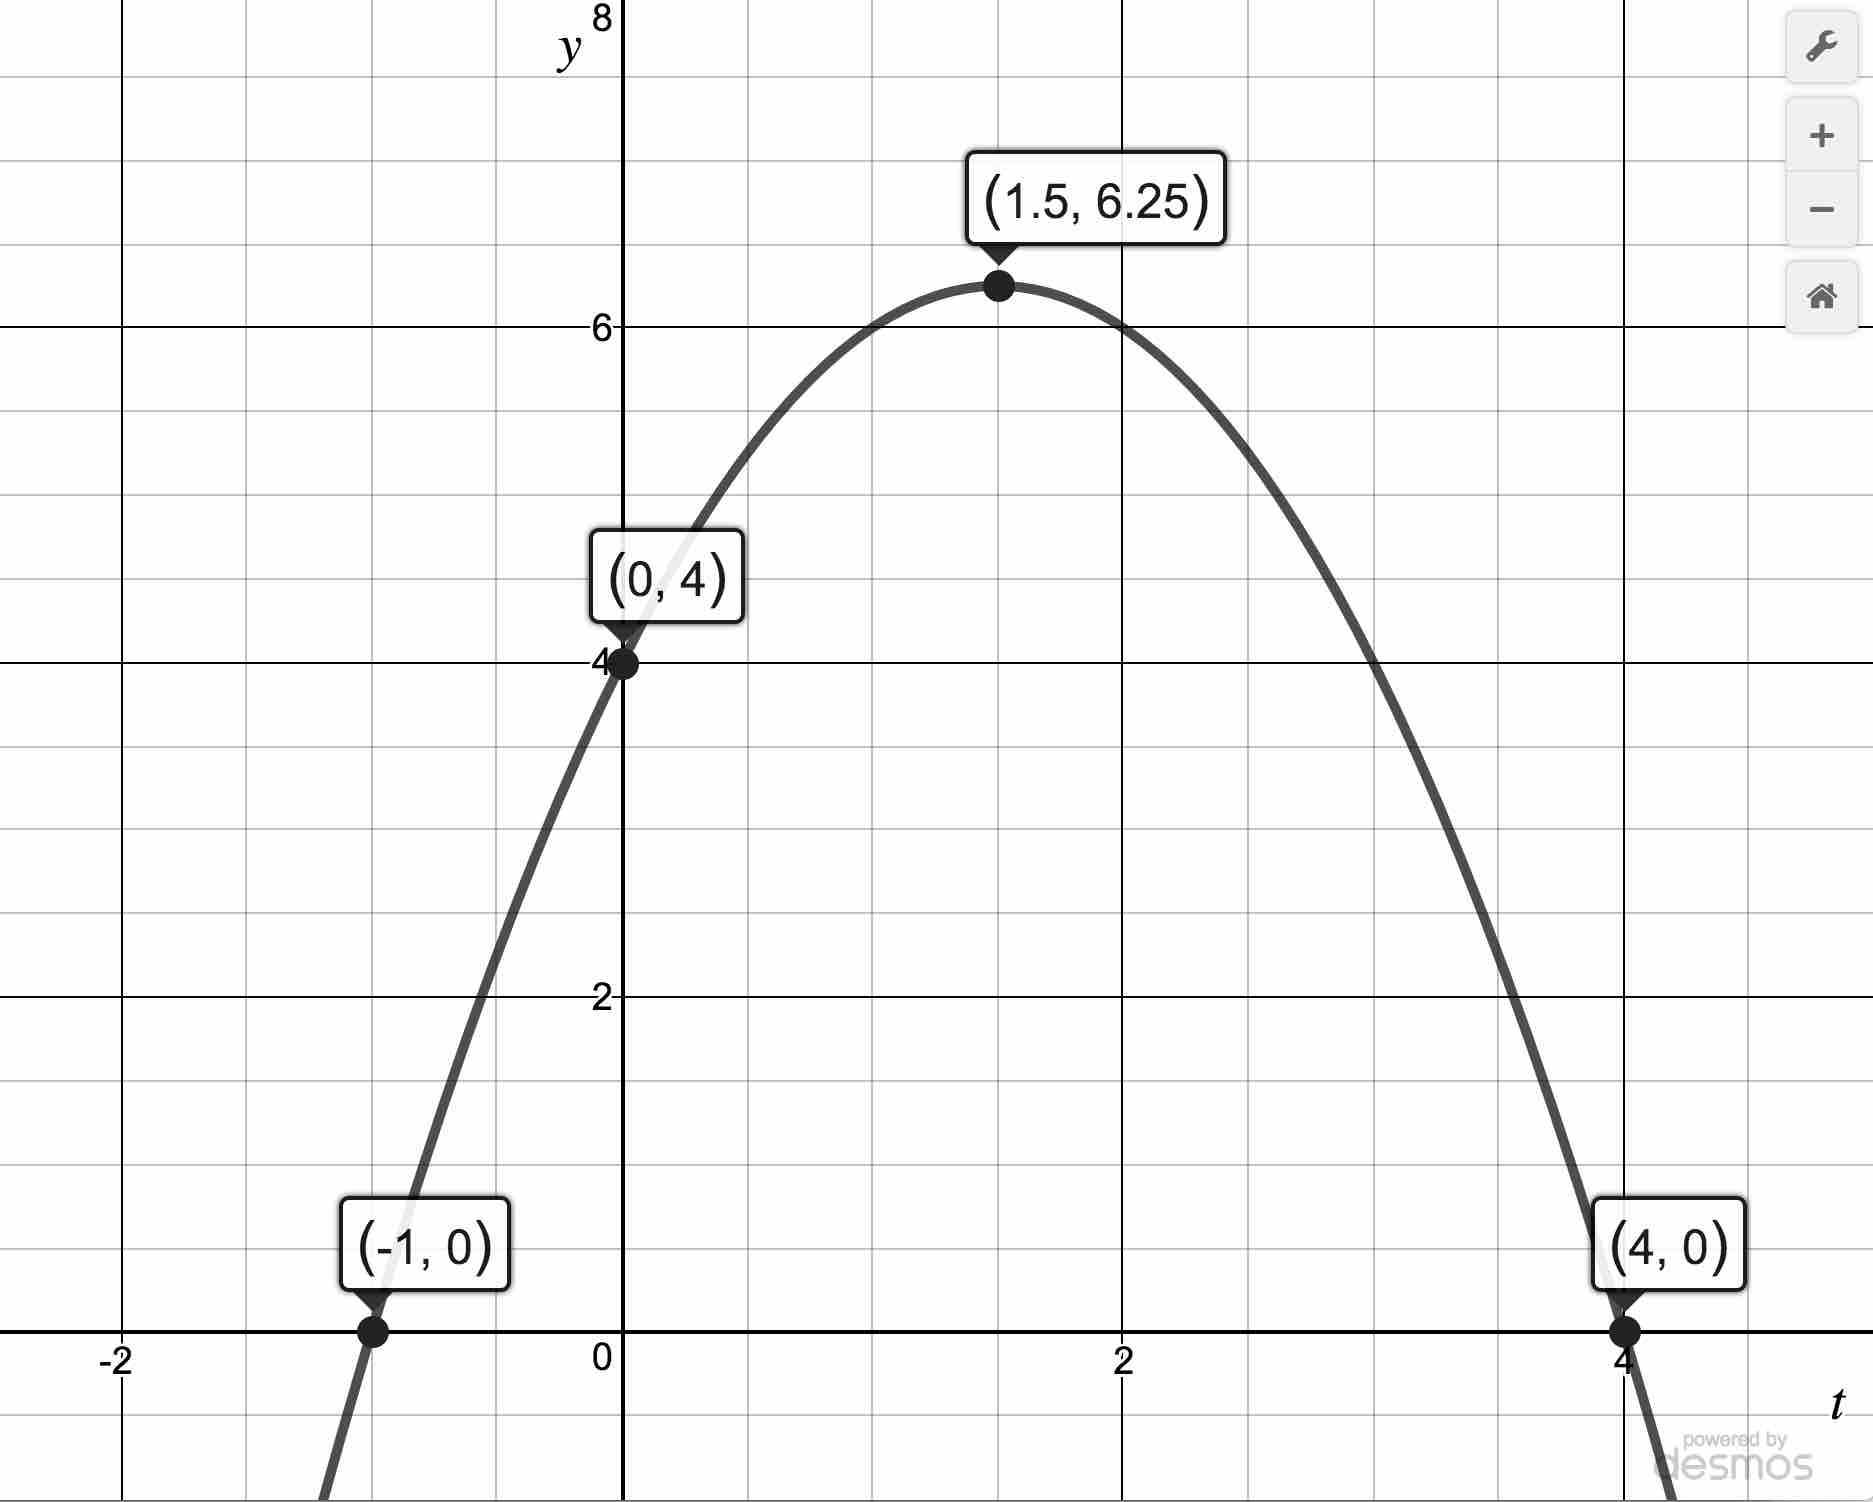
\includegraphics[width=3in]{./FunctionsandtheirRepresentationsGraphics/ParabolaGraph.jpg}

&

\begin{mfpic}[19]{-3}{5}{-2}{7}
\axes
\tlabel[cc](5,-0.5){\scriptsize $t$}
\tlabel[cc](0.5,7){\scriptsize $y$}
\xmarks{-2 step 1 until 4 }
\ymarks{-1 step 1 until 6}
\tlpointsep{5pt}
\scriptsize
\tlabel[cc](-1.75,0.5){$(-1,0)$}
\tlabel[cc](-0.75,4){$(0,4)$}
\tlabel[cc](2.75,6){$(2,6)$}
\tlabel[cc](4.5,0.5){$(4,0)$}
\tlabel[cc](1.5,6.75){$(1.5,6.25)$}

\axislabels {x}{{$-2 \hspace{7pt}$} -2,{$-1 \hspace{7pt}$} -1, {$1$} 1, {$2$} 2, {$3$} 3, {$4$} 4}
\axislabels {y}{{$-1$} -1, {$1$} 1, {$2$} 2, {$3$} 3, {$5$} 5, {$6$} 6}
\normalsize
\penwd{1.5pt}
\arrow \reverse \arrow \function{-1.3,4.3,0.1}{4+3x-x**2}
\point[4pt]{(-1,0), (0,4), (1.5, 6.25), (2,6), (4,0)}
\end{mfpic}  \\

\end{tabular}

\end{center}

\vspace*{-.5in} \qed

\end{ex}

Our last example of the section uses the interplay between algebraic and graphical representations of a function to solve a real-world problem.

\begin{ex} \label{volumeex1}    The United States Postal Service mandates that when shipping parcels using `Parcel Select' service,  the sum of the length (the longest dimension) and the girth (the distance around the thickest part of the parcel perpendicular to the length) must not exceed 130 inches.\footnote{See \href{http://pe.usps.com/text/qsg300/Q201e.htm}{\underline{here}}.}  Suppose we wish to ship a rectangular box whose girth forms a square measuring $x$ inches per side as shown below.

\begin{center}

\begin{mfpic}[10]{-6}{12}{-1}{17}
\polyline{(0,0),(-4,3)}
\polyline{(-4,3), (-4,8)}
\polyline{(-4,8),(0,5)}
\polyline{(0,5),(0,0)}
\polyline{(0,0),(12,9)}
\polyline{(0,5),(12,14)}
\polyline{(-4,8),(8,17)}
\polyline{(8,17),(12,14)}
\polyline{(12,14),(12,9)}%6
\arrow \reverse \arrow \polyline{(0.5,-0.125),(12,8.5)}
\tlabel[cc](9,4){length}
\arrow \reverse \arrow \polyline{(-4, 2.5), (-0.5,-0.125)}
\tlabel[cc](-3,0.5){ $x$}
\arrow \reverse \arrow \polyline{(-4.5, 3), (-4.5,8)}
\tlabel[cc](-5,5){$x$}
\end{mfpic}

\end{center}

It turns out\co{\footnote{We'll skip the explanation for now because we want to focus on just the different representations of the function. Rest assured, you'll be asked to construct this very model in Exercise \ref{girthbox1} in Section \ref{GraphsofPolynomials}.}} that the volume of a box, $V(x)$, measured in cubic inches,  whose length plus girth is exactly 130 inches is given by the formula: $V(x) = x^2 (130-4x)$ for $0 < x \leq 26$.

%\pagebreak

\begin{enumerate}

\item  Find and interpret $V(5)$.

\item  Make a table of values and use these along with a graphing utility to graph $y = V(x)$.

\item  What is the largest volume box that can be shipped?  What value of $x$ maximizes the volume?  Round your answers to two decimal places.

\end{enumerate}
{\bf Solution.}

\begin{enumerate}

\item To find $V(5)$, we substitute $x=5$ into the expression $V(x)$:  $V(5) = (5)^2 (130-4(5)) = 25(110) = 2750$.   Our result means that when the length and width of the square  measure $5$ inches, the volume of the resulting box is $2750$ cubic inches.\footnote{Note that we have $V(5)$ and $25(110)$ in the same string of equality. The first set of parentheses is function notation and directs us to substitute $5$ for $x$ in the expression $V(x)$ while the second indicates multiplying $25$ by $110$. Context is key!}

\item The domain of $V$ is specified by the inequality  $0 < x \leq 26$, so we can begin graphing $V$ by sampling  $V$ at finitely many $x$-values in this interval to help us get a sense of the range of $V$. This, in turn, will help us determine an adequate viewing window on our graphing utility when the time comes.

It seems natural to start with what's happening near $x = 0$.  Even though the expression $x^2 (130-4x)$  is defined when we substitute $x = 0$ (it reduces very quickly to $0$), it would be incorrect to state $V(0) = 0$ because $x = 0$ is not in the domain of $V$.  However,  there is nothing stopping us from evaluating $V(x)$ at values $x$ `very close' to $x = 0$.  A table of such values is given below. \[ \begin{array}{||l|l||} \hline 
        x & V(x) \\ \hline
      0.1 & 1.296 \\ \hline
     0.01 & 0.012996 \\ \hline
    0.001 & 0.000129996 \\ \hline
10^{-23} & \approx 1.3 \times 10^{-44} \\ \hline

\end{array} \] There is no such thing as a  `smallest' positive number,\footnote{If $p$ is any positive real number, $0 < 0.5 p < p$, so we can always find a smaller positive real number.}  so we will have points on the graph of $V$ to the right of $x = 0$ leading to the point $(0,0)$.  We indicate this behavior by putting a hole at $(0,0)$.\footnote{What's really needed here is the precise definition of `closeness' discussed in Calculus.  This hand-waving will do for now.}

Moving forward, we start with $x = 5$ and sample $V$ at steps of $5$ in its domain.  Our goal is to graph $y = V(x)$, so we plot our points $(x, V(x))$  using  the domain as a guide to help us set the horizontal bounds (i.e., the bounds on $x$) and the sample values from the range to help us set the vertical bounds (i.e., the bounds on $y$).   The right endpoint, $x = 26$, is included in the domain $0 < x \leq 26$ so we finish the graph by plotting the point $(26, V(26)) = (26,17576)$.  At the top of the next page on the left is the table of data and on the right is a graph produced with some help from \href{https://www.desmos.com/}{\underline{desmos}}.
  
\begin{tabular}{m{1.9 in}m{4in}}

$\begin{array}{|r||c|c|}  \hline

  x & V(x) & (x,V(x)) \\ \hline
  
\approx 0 & \approx 0  & \text{hole at $(0,0)$} \\  \hline
 5 & 2750 & (5, 2750) \\  \hline
 10 & 9000 & (10, 9000) \\  \hline
 15 & 15, \! 750 & ( 15, 15, \! 750) \\  \hline
  20 & 20, \! 000 & ( 20 , 20, \! 000) \\  \hline
  25 & 18, \! 750 & ( 25, 18, \! 750) \\  \hline
  26 & 17, \! 576 &  (26,17, \! 576) \\ \hline
\end{array}$

&

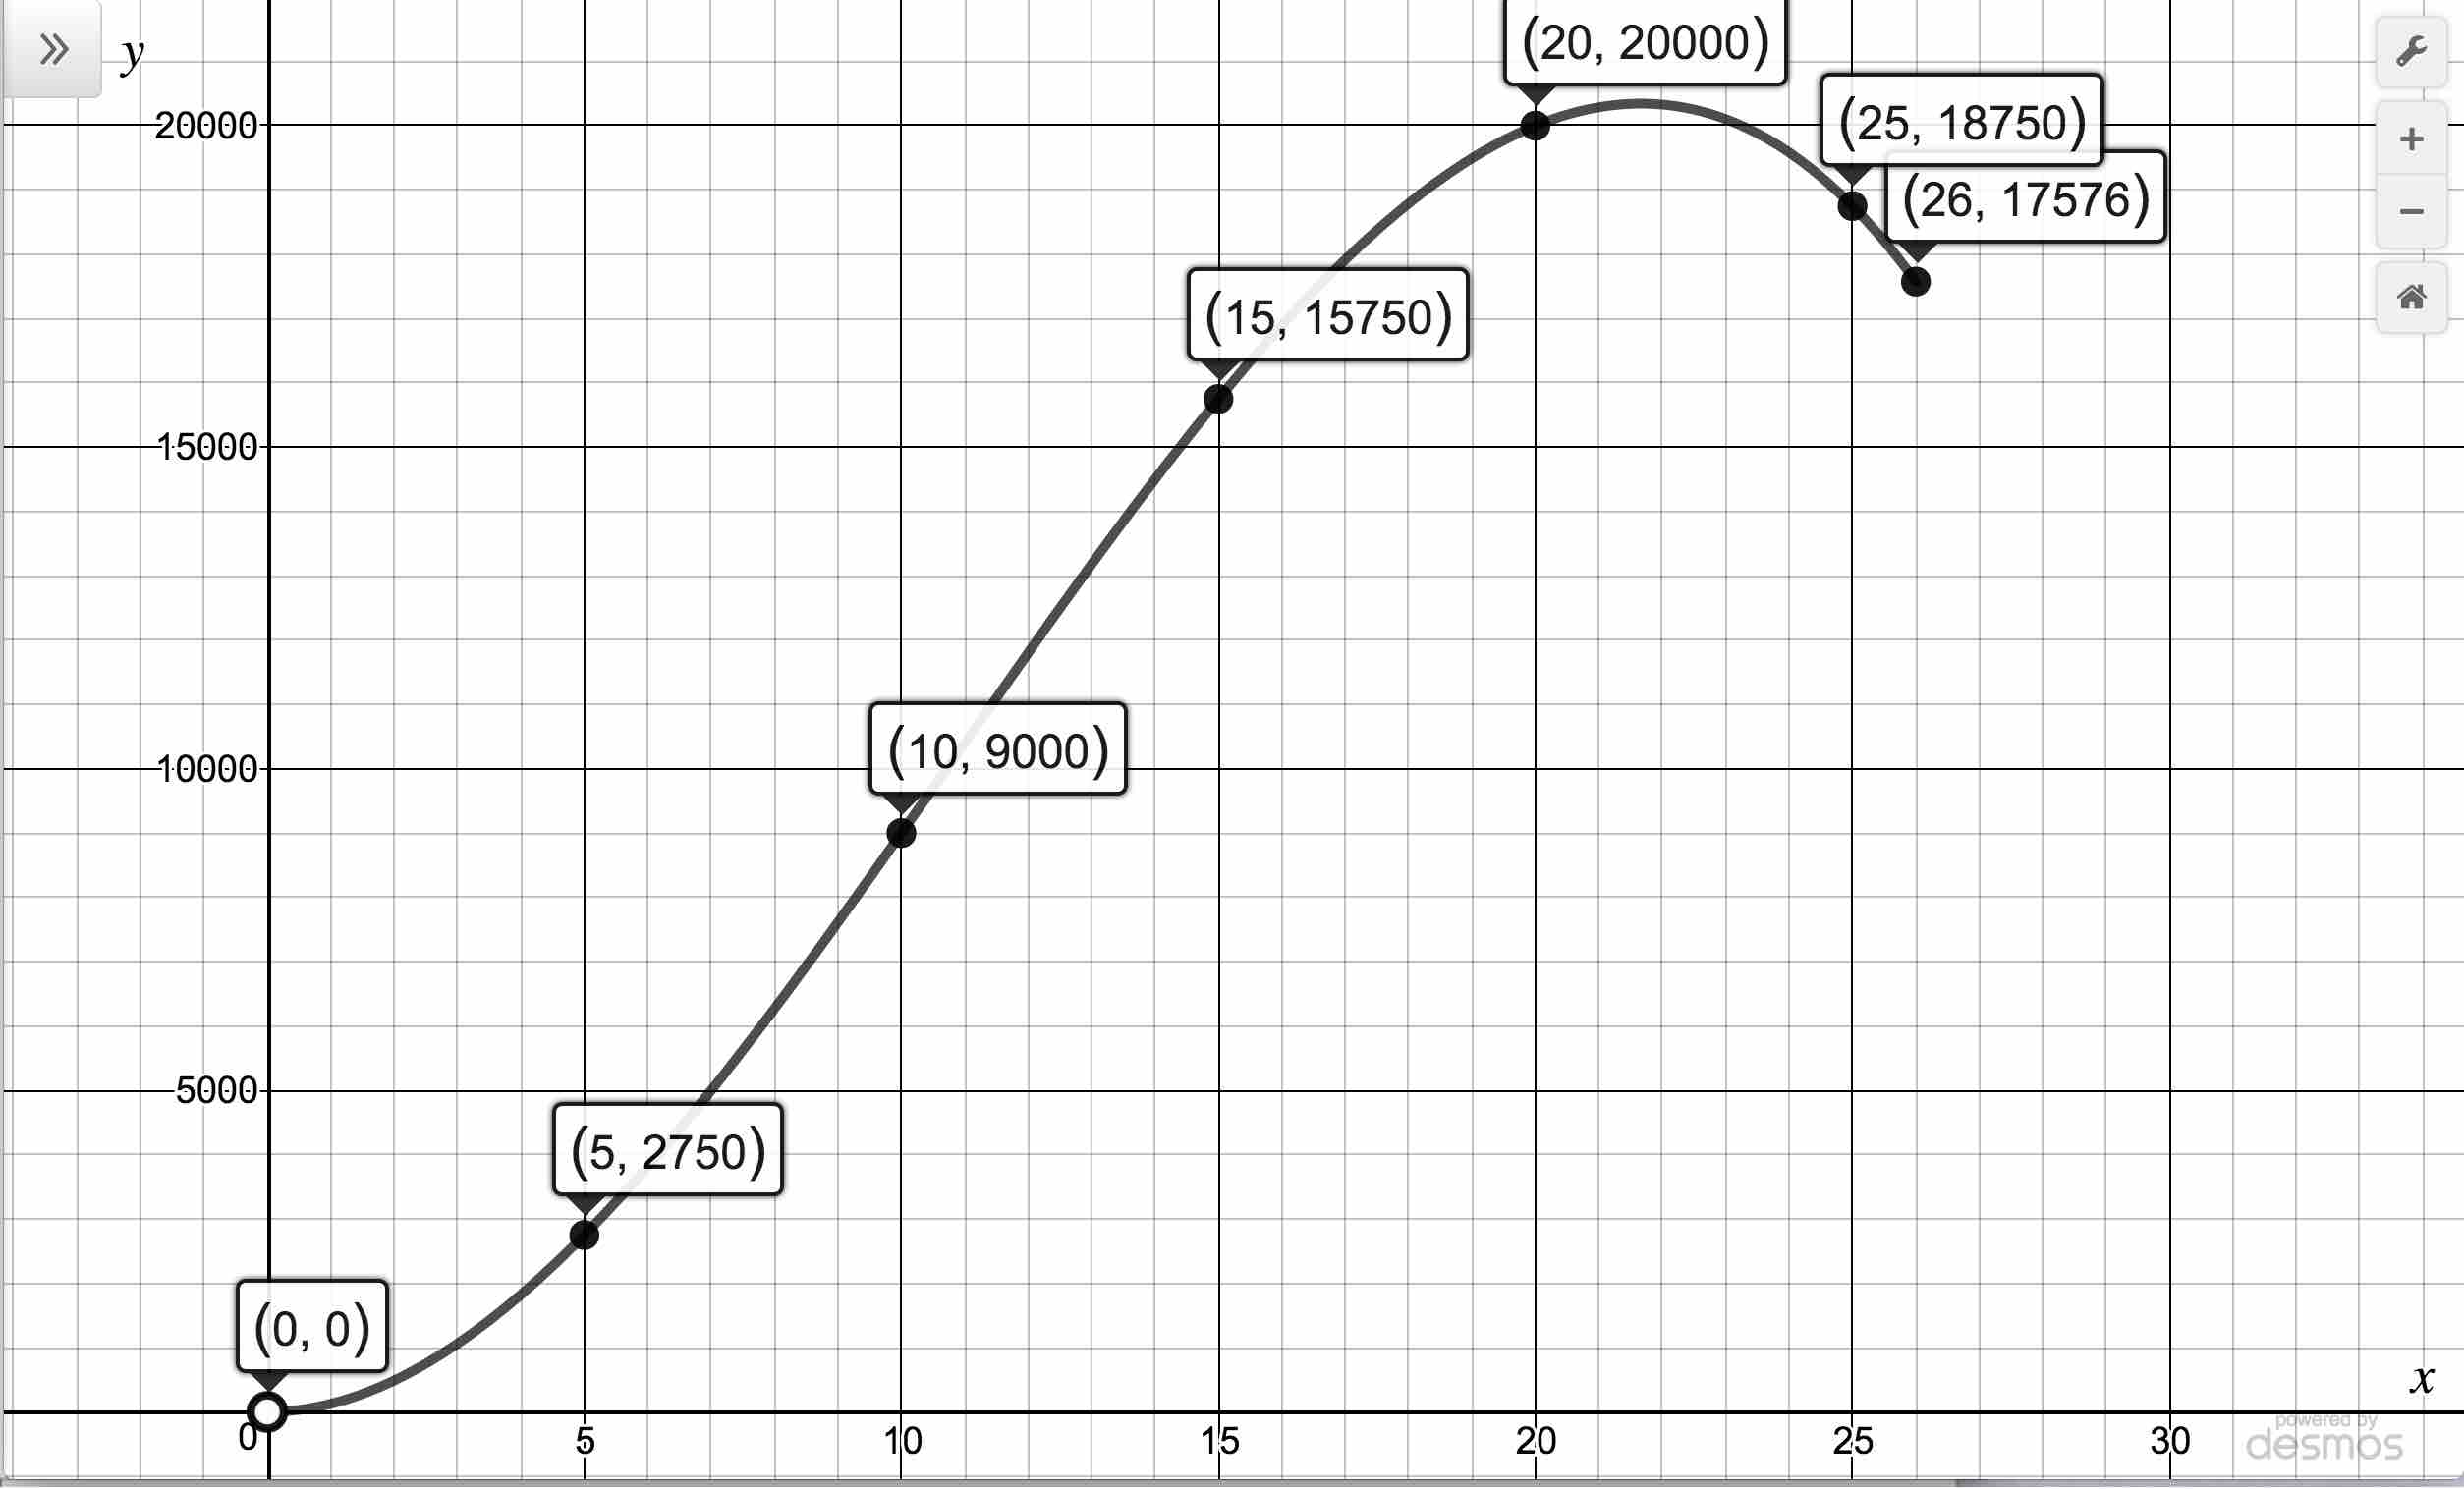
\includegraphics[width=4in]{./FunctionsandtheirRepresentationsGraphics/VolumeEx01.jpg}  \\

\centerline{Sampling $V$}

&

\centerline{The graph of $y = V(x)$}

\end{tabular}


\item  The largest volume in this case refers to the maximum of $V$.  The biggest $y$-value in our table of data is $20, \! 000$ cubic inches which occurs at $x = 20$ inches, but the graph produced by the graphing utility indicates that there are points on the graph of $V$ with $y$-values (hence $V(x)$ values) greater than $20, \! 000$.  Indeed, the graph continues to rise to the right of $x = 20$ and the graphing utility reports the maximum $y$-value to be $y \approx 20, \! 342.593$ when $x \approx 21.667$.  Rounding to two decimal places, we find the maximum volume obtainable under these conditions is about $20, \! 342.59$ cubic inches which occurs when the length and width of the square side of the box are approximately $21.67$ inches.\footnote{We could also find the length of the box in this case as well.  The sum of length and girth is 130 inches so the length is 130 minus the girth, or $130 - 4x \approx 130 - 4(21.67) = 43.32$ inches.}  

\begin{center}

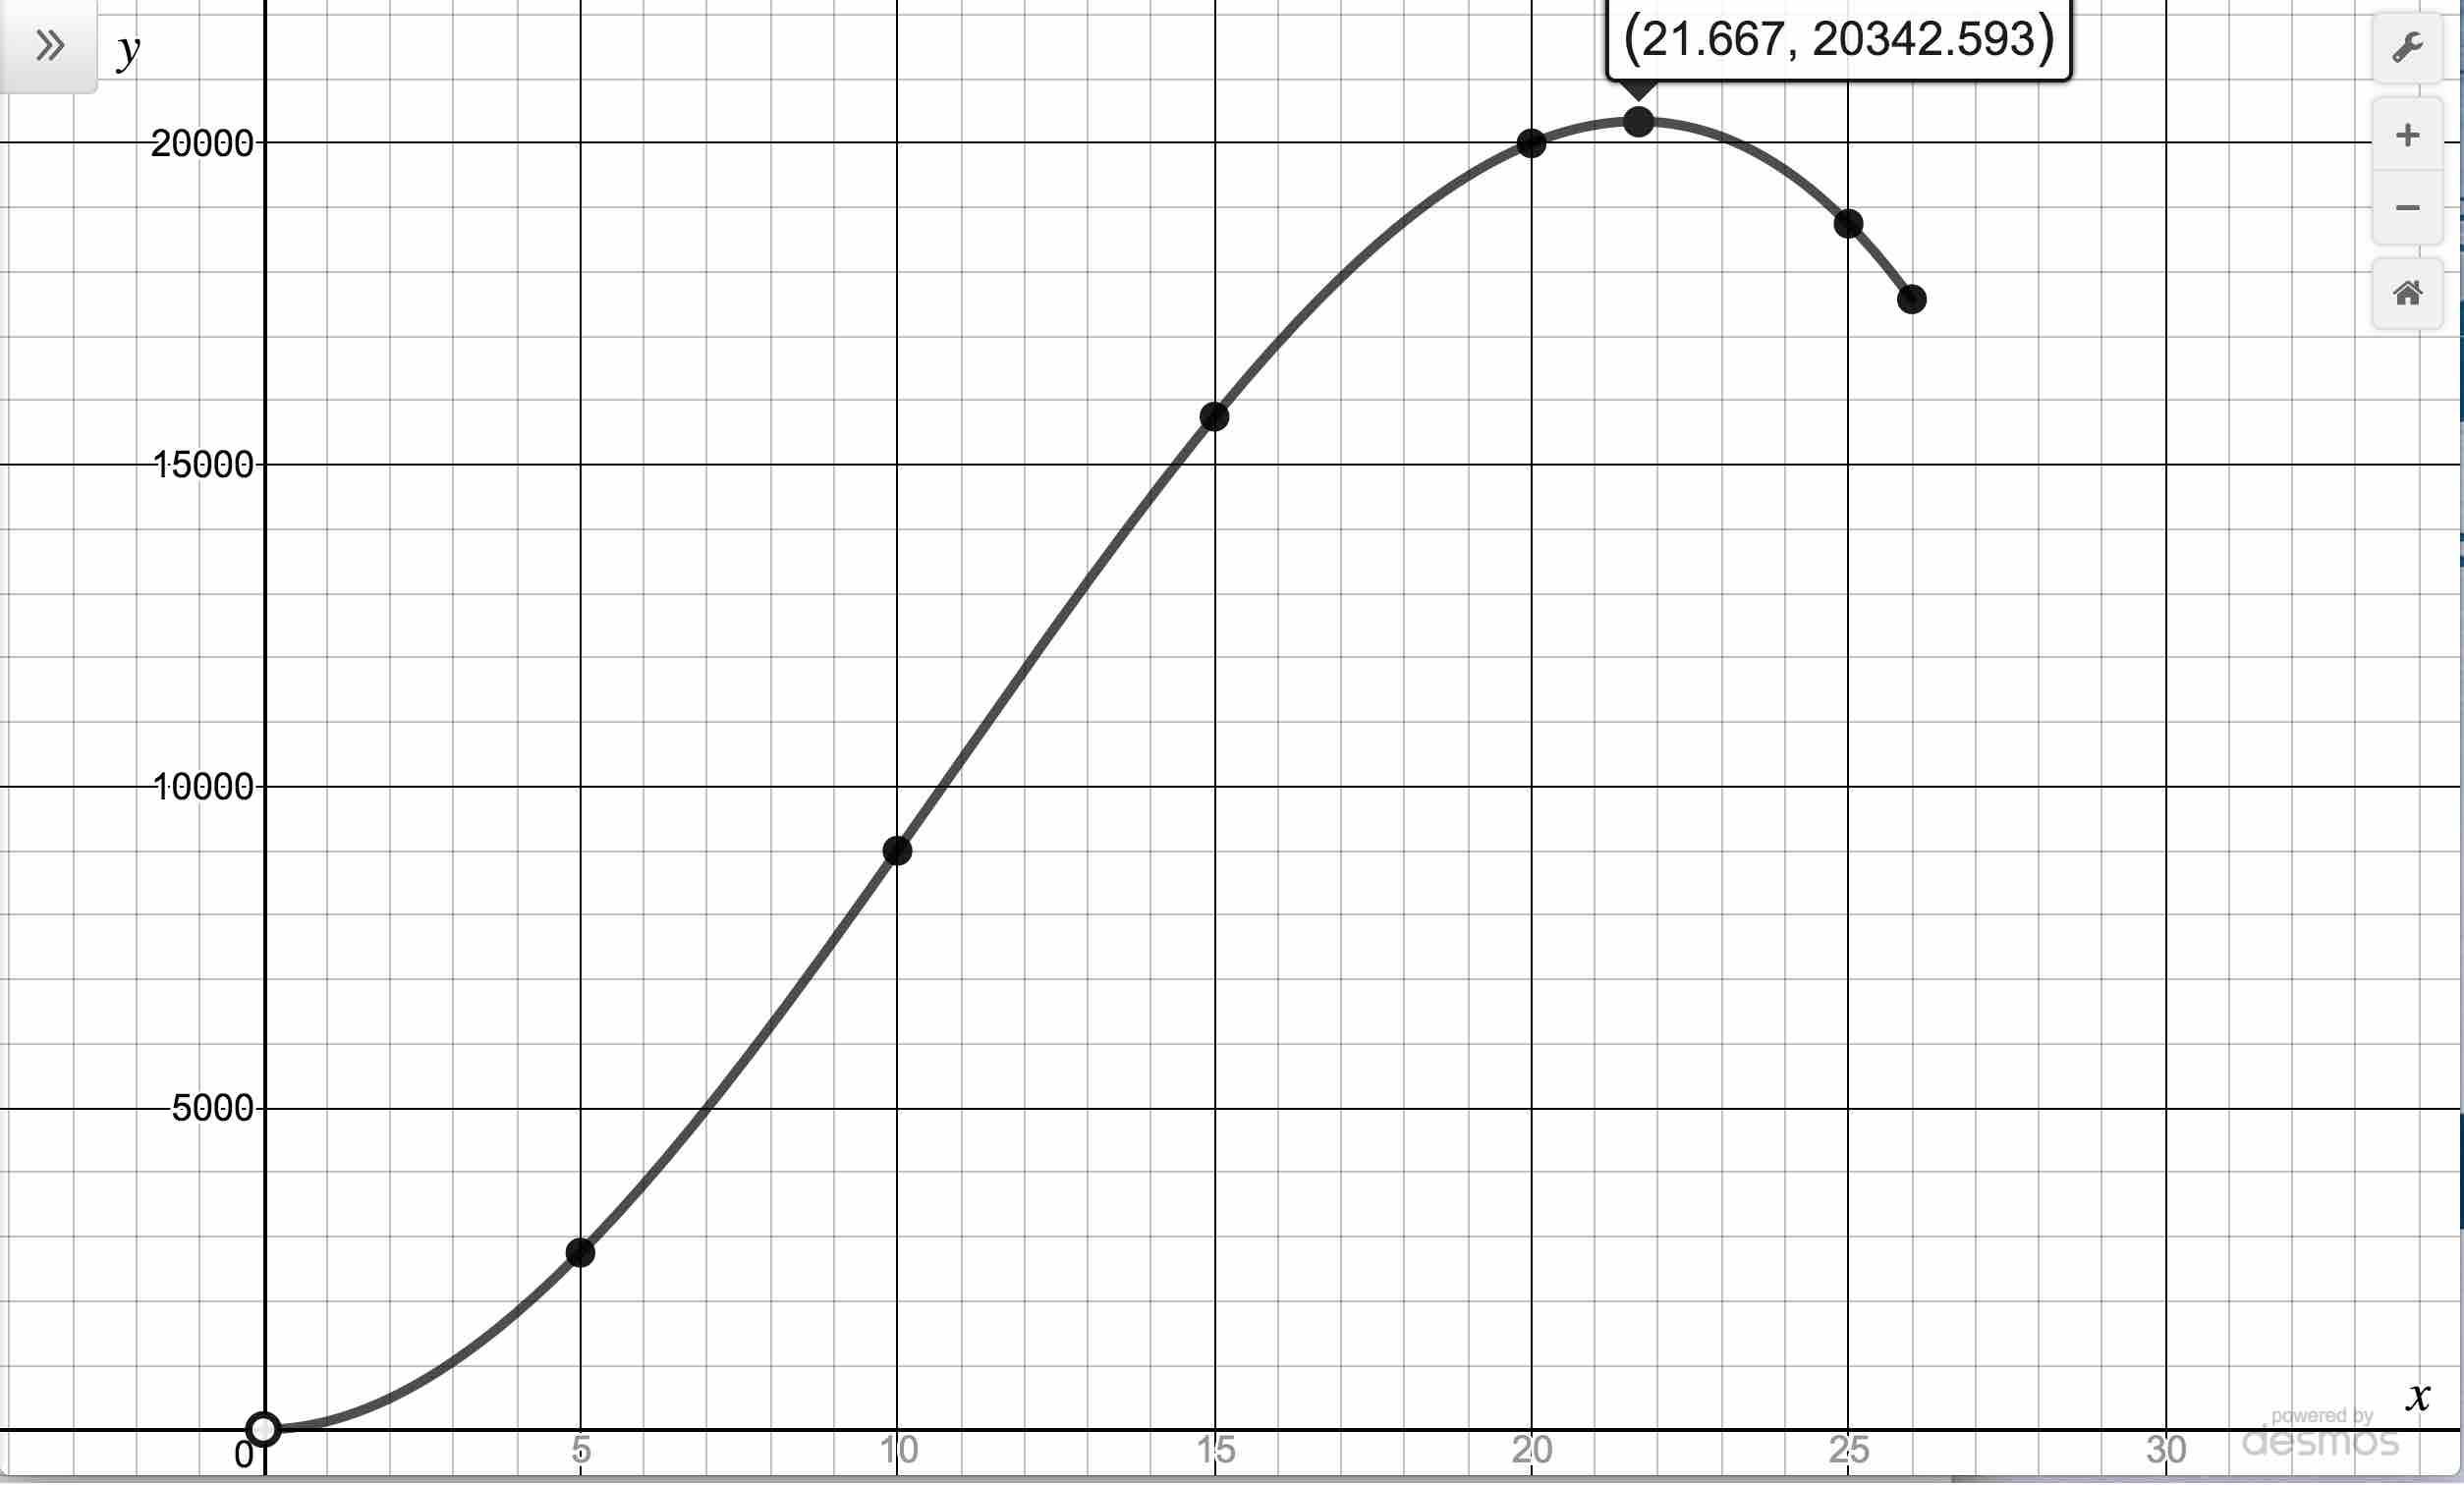
\includegraphics[width=4in]{./FunctionsandtheirRepresentationsGraphics/VolumeEx02.jpg} 

Finding the maximum volume using the graph of $y = V(x)$.

\end{center}

%\pagebreak

It is worth noting that while the function $V$ has a maximum, it did not have a minimum.  Even though $V(x)>0$ for all $x$ in its domain,\footnote{said differently, the values of $V(x)$ are \textbf{bounded below} by $0$.} the presence of the hole at $(0,0)$ means that $0$ is not in the range of $V$.  Hence, based on our model, we can never make a box with a  `smallest' volume.\footnote{How realistic is this?}  \qed

\end{enumerate}
\end{ex}

\medskip

Example \ref{volumeex1} typifies the interplay between Algebra and Geometry which lies ahead.  Both the algebraic description of  $V$: $V(x) = x^2 (130 - 4x)$ for $0 < x \leq 26$, and the graph of $y=V(x)$ were useful in describing aspects of the physical situation at hand.  Wherever possible, we'll use the algebraic representations of functions to \textit{analytically} produce \textit{exact} answers to certain problems and use the graphical descriptions to check the reasonableness of our answers. 

\medskip

That being said, we'll also encounter problems which we simply \textit{cannot} answer analytically (such as determining the maximum volume in the previous example), so we will be forced to resort to using technology (specifically graphing technology) in order to find \textit{approximate} solutions.  The most important thing to keep in mind is that while technology may \textit{suggest} a result, it is ultimately Mathematics that \textit{proves} it. 

\medskip

We close this section with a summary of the different ways to represent functions.

\bigskip

\colorbox{ResultColor}{\bbm
\begin{boxinfo}
\centerline{\textbf{Ways to Represent a Function}} \label{waystorepresentfunctionsbox}

\smallskip

Suppose $f$ is a function with domain $A$.  Then $f$ can be represented:

\begin{itemize}

\item  verbally; that is, by describing how the inputs are matched with their outputs.

\item using a mapping diagram.

\item  as a set of ordered pairs of the form $(\text{input}, \text{output})$:  $\{ (a, f(a)) \, | \, a \in A \}$.

\end{itemize}

If $f$ is a function whose domain and range are subsets of real numbers, then $f$ can be represented:

\begin{itemize}

\item  algebraically as a formula for $f(a)$.

\item  graphically by plotting the points $\{ (a, f(a))  \, | \, a \in A \}$ in the plane.

\end{itemize}

Note: An important consequence of the last bulleted item is that the point $(a, b)$ is on the graph of $y = f(x)$ if and only if $f(a) = b.$\label{FundamentalGraphingPrinciple}
\end{boxinfo}
\ebm}

\newpage

\subsection{Exercises}
In Exercises \ref{mappingfirst} - \ref{mappinglast}, determine whether or not the mapping diagram represents a function. Explain your reasoning. If the mapping does represent a function, state the domain, range, and represent the function as a set of ordered pairs.

\begin{multicols}{2}

\begin{enumerate}


\item  \label{mappingfirst} 

$~$

\begin{mfpic}[19]{-5}{5}{-5}{6}
\tlabel[cc](-4.25,5){Tennant}
\tlabel[cc](-4.25,3){Smith}
\tlabel[cc](-4.25,1){Calpadi}
\tlabel[cc](0,6){$M$}
\tlabel[cc](3.5,5){Eleven}
\tlabel[cc](3.5,3){Twelve}
\tlabel[cc](3.5,1){Thirteen}
\tlabel[cc](3.5,-1){Fourteen}
\arrow[l 5pt] \polyline{(-2.5, 5), (2.5, 5)}
\arrow[l 5pt] \polyline{(-2.5, 5), (2.5, 3)}
\arrow[l 5pt] \polyline{(-2.5, 3), (2.5, 1)}
\arrow[l 5pt] \polyline{(-2.5, 1), (2.5, -1)}
\end{mfpic} 



\item  \label{mappinglast} 

$~$

\begin{mfpic}[19]{-5}{5}{-5}{6}
\tlabel[cc](-4.25,5){Hartnell}
\tlabel[cc](-4.25,3){Cushing}
\tlabel[cc](-4.25,1){Hurndall}
\tlabel[cc](-4.25,-1){Troughton}
\tlabel[cc](0,6){$C$}
\tlabel[cc](3.5,5){One}
\tlabel[cc](3.5,3){Two}
\tlabel[cc](3.5,1){Three}
\arrow[l 5pt] \polyline{(-2.5, 5), (2.5, 5)}
\arrow[l 5pt] \polyline{(-2.5, 3), (2.5, 5)}
\arrow[l 5pt] \polyline{(-2.5, 1), (2.5, 5)}
\arrow[l 5pt] \polyline{(-2.5, -1), (2.5, 3)}
\end{mfpic}

\setcounter{HW}{\value{enumi}}

\end{enumerate}

\end{multicols}

In Exercises \ref{tablefirst} - \ref{tablelast}, determine whether or not the data in the given table represents $y$ as a function of $x$.  Explain your reasoning.  If the mapping does represent a function, state the domain, range, and represent the function as a set of ordered pairs.

\begin{multicols}{2}

\begin{enumerate}

\setcounter{enumi}{\value{HW}}

\item  \label{tablefirst} 

\[\begin{array}{|r||r|}  \hline

$x$  & \hphantom{\text{$-$}} $y$  \\ \hline
 -3 &  3 \\  \hline
 -2 & 2  \\  \hline
  -1 &  1  \\  \hline
 0 &  0 \\  \hline
 1 & 1  \\  \hline
 2 &  2 \\  \hline
 3 & 3  \\  \hline

\end{array}\]

\item \label{tablelast}

\[\begin{array}{|r||r|}  \hline

\hphantom{\text{$-$}} $x$  &$y$  \\ \hline

 0 & 0 \\  \hline
 1 & 1  \\  \hline
 1 & -1  \\  \hline
 2 &  2 \\  \hline
 2 & -2  \\  \hline
 3 &  3 \\  \hline
 3 & -3  \\  \hline

\end{array}\]

\setcounter{HW}{\value{enumi}}

\end{enumerate}

\end{multicols}

\begin{enumerate}

\setcounter{enumi}{\value{HW}}

\item    Suppose $W$ is the set of words in the English language and we set up a mapping from $W$ into the set of natural numbers $\mathbb{N}$ as follows: $\text{word} \rightarrow \text{number of letters in the word}$.  Explain why this mapping is a function.  What would you need to know to determine the range of the function?

\item  Suppose $L$ is the set of last names of all the people who have served or are currently serving as the President of the United States.   Consider the mapping from $L$ into $\mathbb{N}$ as follows:  $\text{last name} \rightarrow \text{number of their presidency}$.  For example,  $\text{Washington} \rightarrow 1$ and $\text{Obama} \rightarrow 44$.  Is this mapping a function?  What if we use full names instead of just last names? (\textbf{HINT:}  Research Grover Cleveland.)

\item  Under what conditions would the time of day be a function of the outdoor temperature?

\setcounter{HW}{\value{enumi}}

\end{enumerate}


For the functions $f$ described in Exercises \ref{buildfunctionfirst} - \ref{buildfunctionlast}, find $f(2)$ and find and simplify an expression for $f(x)$ that takes a real number $x$ and performs the following three steps in the order given: 


\begin{enumerate}
\setcounter{enumi}{\value{HW}}

\item  (1) multiply by 2; (2) add 3; (3) divide by 4. \label{buildfunctionfirst}

\item  (1) add 3; (2) multiply by 2; (3) divide by 4. 

\item (1) divide by 4; (2) add 3; (3) multiply by 2.

\item (1) multiply by 2; (2) add 3; (3) take the square root.

\item  (1) add 3; (2) multiply by 2; (3) take the square root.

\item  (1) add 3; (2) take the square root; (3) multiply by 2.  \label{buildfunctionlast}

\setcounter{HW}{\value{enumi}}
\end{enumerate}


In Exercises \ref{funcnotationbasicfirst} - \ref{funcnotationbasiclast}, use the given function $f$ to find and simplify the following:

\begin{multicols}{3}
\begin{itemize}
\item $f(3)$
\item $f(-1)$
\item $f\left(\frac{3}{2} \right)$
\end{itemize}
\end{multicols}

\begin{multicols}{3}
\begin{itemize}
\item  $f(4x)$
\item $4f(x)$
\item $f(-x)$
\end{itemize}
\end{multicols}

\begin{multicols}{3}
\begin{itemize}
\item  $f(x-4)$
\item $f(x) - 4$
\item  $f\left(x^2\right)$
\end{itemize}
\end{multicols}

\begin{multicols}{2}
\begin{enumerate}
\setcounter{enumi}{\value{HW}}

\item  $f(x) = 2x+1$ \label{funcnotationbasicfirst} 
\item  $f(x) = 3 - 4x$

\setcounter{HW}{\value{enumi}}
\end{enumerate}
\end{multicols}

\begin{multicols}{2}
\begin{enumerate}
\setcounter{enumi}{\value{HW}}

\item $f(x) = 2 - x^2$
\item $f(x) = x^2 - 3x + 2$

\setcounter{HW}{\value{enumi}}
\end{enumerate}
\end{multicols}


\begin{multicols}{2}
\begin{enumerate}
\setcounter{enumi}{\value{HW}}

\item $f(x) = 6$
\item $f(x) = 0$ \label{funcnotationbasiclast}

\setcounter{HW}{\value{enumi}}
\end{enumerate}
\end{multicols}

In Exercises \ref{secondfuncnotationbasicfirst} - \ref{secondfuncnotationbasiclast}, use the given function $f$ to find and simplify the following:

\begin{multicols}{3}
\begin{itemize}

\item  $f(2)$
\item  $f(-2)$
\item  $f(2a)$

\end{itemize}
\end{multicols}

\begin{multicols}{3}
\begin{itemize}

\item  $2 f(a)$
\item $f(a+2)$
\item $f(a) + f(2)$

\end{itemize}
\end{multicols}

\begin{multicols}{3}
\begin{itemize}

\item  $f \left( \dfrac{2}{a} \right)$
\item $\dfrac{f(a)}{2}$
\item  $f(a + h)$

\end{itemize}
\end{multicols}


\begin{multicols}{2}
\begin{enumerate}
\setcounter{enumi}{\value{HW}}

\item $f(x) = 2x-5$ \label{secondfuncnotationbasicfirst}
\item $f(t) = 5-2t$

\setcounter{HW}{\value{enumi}}
\end{enumerate}
\end{multicols}

\begin{multicols}{2}
\begin{enumerate}
\setcounter{enumi}{\value{HW}}

\item $f(w) = 2w^2 - 1$
\item $f(q) = 3q^2+3q-2$

\setcounter{HW}{\value{enumi}}
\end{enumerate}
\end{multicols}
 
\begin{multicols}{2}
\begin{enumerate}
\setcounter{enumi}{\value{HW}}


\item $f(r) = 117$
\item $f(z) = \dfrac{z}{2}$  \label{secondfuncnotationbasiclast}

\setcounter{HW}{\value{enumi}}
\end{enumerate}
\end{multicols}


%\newpage


In Exercises \ref{findzerofuncfirst} - \ref{findzerofunclast}, use the given function $f$ to find $f(0)$ and solve $f(x) = 0$

\begin{multicols}{2}
\begin{enumerate}
\setcounter{enumi}{\value{HW}}

\item $f(x) = 2x - 1$ \label{findzerofuncfirst}
\item $f(x) = 3 - \frac{2}{5} x$

\setcounter{HW}{\value{enumi}}
\end{enumerate}
\end{multicols}

\begin{multicols}{2}
\begin{enumerate}
\setcounter{enumi}{\value{HW}}

\item $f(x) = 2x^2 - 6$
\item $f(x) = x^2 - x - 12$ \label{findzerofunclast}

\setcounter{HW}{\value{enumi}}
\end{enumerate}
\end{multicols}


In Exercises \ref{equfunctionfirst} - \ref{equfunctionlast}, determine whether or not the equation represents $y$ as a function of $x$.  



\begin{multicols}{3}
\begin{enumerate}
\setcounter{enumi}{\value{HW}}

\item $y = x^{3} - x$ \label{equfunctionfirst}
\item $y = \sqrt{x - 2}$
\item $x^{3}y = -4$ 
\setcounter{HW}{\value{enumi}}
\end{enumerate}
\end{multicols}

\begin{multicols}{3}
\begin{enumerate}
\setcounter{enumi}{\value{HW}}

\item $x^{2} - y^{2} = 1$
\item $y = \dfrac{x}{x^{2} - 9}$
\item $x = -6$

\setcounter{HW}{\value{enumi}}
\end{enumerate}
\end{multicols}

\begin{multicols}{3}
\begin{enumerate}
\setcounter{enumi}{\value{HW}}

\item  $x = y^2 + 4$

\item $y = x^2 + 4$
\item $x^2 + y^2 = 4$

\setcounter{HW}{\value{enumi}}
\end{enumerate}
\end{multicols}

\begin{multicols}{3}
\begin{enumerate}
\setcounter{enumi}{\value{HW}}


\item $y = \sqrt{4-x^2}$
\item $x^2 - y^2 = 4$
\item $x^3 + y^3 = 4$


\setcounter{HW}{\value{enumi}}
\end{enumerate}
\end{multicols}

\begin{multicols}{3}
\begin{enumerate}
\setcounter{enumi}{\value{HW}}

\item $2x + 3y = 4$
\item $2xy = 4$
\item $x^2 = y^2$ \label{equfunctionlast}

\setcounter{HW}{\value{enumi}}
\end{enumerate}
\end{multicols}





Exercises \ref{setfunctionfirst} - \ref{setfunctionlast} give a set of points in the $xy$-plane.    Determine if $y$ is a function of $x$.  If so, state the domain and range.

\begin{enumerate}

\setcounter{enumi}{\value{HW}}

\item \{$(-3, 9)$, $\;(-2, 4)$, $\;(-1, 1)$, $\;(0, 0)$, $\;(1, 1)$, $\;(2, 4)$, $\;(3, 9)\}$ \label{setfunctionfirst}
\item  $\left\{ (-3,0), (1,6), (2, -3), (4,2), (-5,6), (4, -9), (6,2) \right\}$
\item  $\left\{ (-3,0), (-7,6), (5,5), (6,4), (4,9), (3,0) \right\}$
\item  $\left\{ (1,2), (4,4), (9,6), (16,8), (25,10), (36, 12), \ldots \right\}$
\item \{($x, y) \, | \, x$ is an odd integer, and $y$ is an even integer\}
\item \{$(x, 1) \, | \, x$ is an irrational number\}

\item $\{ (1,0), (2,1), (4,2), (8,3), (16,4), (32, 5), \ldots \}$
\item $\{ \ldots (-3,9), (-2,4), (-1,1), (0,0), (1,1), (2,4), (3,9), \ldots \}$

\setcounter{HW}{\value{enumi}}
\end{enumerate}

\vspace{-0.1in}

\begin{multicols}{2}
\begin{enumerate}
\setcounter{enumi}{\value{HW}}

\item $\{ (-2, y) \, | \, -3 < y < 4\}$
\item  $\{ (x,3) \, | \,  -2 \leq x < 4\}$

\setcounter{HW}{\value{enumi}}
\end{enumerate}
\end{multicols}

\begin{multicols}{2}
\begin{enumerate}
\setcounter{enumi}{\value{HW}}


\item  $\{ \left(x,x^2\right) \, | \, \text{$x$ is a real number} \}$
\item  $\{ \left(x^2,x\right) \, | \, \text{$x$ is a real number} \}$ \label{setfunctionlast}

\setcounter{HW}{\value{enumi}}
\end{enumerate}
\end{multicols}

\begin{enumerate}
\setcounter{enumi}{\value{HW}}

\item  \label{HLTExercise} The Vertical Line Test is a quick way to determine from a graph if the vertical axis variable is a function of the horizontal axis variable. If we are given a graph and asked to determine if the horizontal axis variable is a function of the vertical axis variable, we can use horizontal lines instead of vertical lines to check.  Using Theorem \ref{VLT} as a guide,  formulate a `Horizontal Line Test.'  (We'll refer back to this exercise in Section \ref{InverseFunctions}.)

\setcounter{HW}{\value{enumi}}
\end{enumerate}

%\newpage


In Exercises \ref{graphfunctionfirstxy} - \ref{graphfunctionlastxy}, determine whether or not the graph suggests $y$ is a function of $x$.  For the ones which do, state the domain and range. 

\begin{multicols}{2}
\begin{enumerate}
\setcounter{enumi}{\value{HW}}

\item $~$ \vspace{-.1in} \label{graphfunctionfirstxy}

\begin{mfpic}[17]{-5}{2}{-2}{5}
\point[4pt]{(-4, -1), (-3, 0), (-2, 1), (-1, 2), (0, 3), (1, 4)}
\axes
\tlabel[cc](2,-0.5){\scriptsize $x$}
\tlabel[cc](0.5,4.75){\scriptsize $y$}
\xmarks{-4,-3,-2,-1,1}
\ymarks{-1,1,2,3,4}
\tlpointsep{4pt}
\axislabels {x}{{\tiny $-4 \hspace{8pt}$} -4, {\tiny $-3 \hspace{8pt}$} -3, {\tiny $-2 \hspace{8pt}$} -2, {\tiny $-1 \hspace{8pt}$} -1, {\tiny $1$} 1}
\axislabels {y}{{\tiny $-1$} -1, {\tiny $1$} 1, {\tiny $2$} 2, {\tiny $3$} 3, {\tiny $4$} 4}
\end{mfpic}

\vfill
\columnbreak

\item $~$  \label{graphfunctionfirstxy2}

\begin{mfpic}[15]{-5}{2}{-2}{5}
\point[4pt]{(-4, -1), (-3, 0), (-3, 1), (-2, 1), (-1, 2), (0, 3), (1, 4)}
\axes
\tlabel[cc](2,-0.5){\scriptsize $x$}
\tlabel[cc](0.5,4.75){\scriptsize $y$}
\xmarks{-4,-3,-2,-1,1}
\ymarks{-1,1,2,3,4}
\tlpointsep{4pt}
\axislabels {x}{{\tiny $-4 \hspace{6pt}$} -4, {\tiny $-3 \hspace{6pt}$} -3, {\tiny $-2 \hspace{6pt}$} -2, {\tiny $-1 \hspace{6pt}$} -1, {\tiny $1$} 1}
\axislabels {y}{{\tiny $-1$} -1, {\tiny $1$} 1, {\tiny $2$} 2, {\tiny $3$} 3, {\tiny $4$} 4}
\end{mfpic}


\setcounter{HW}{\value{enumi}}
\end{enumerate}
\end{multicols}


\begin{multicols}{2}
\begin{enumerate}
\setcounter{enumi}{\value{HW}}



\item $~$ \label{graphfunctionfirstxy3}

\begin{mfpic}[15]{-3}{3}{-1}{6}
\axes
\tlabel[cc](3,-0.5){\scriptsize $x$}
\tlabel[cc](0.5,5.75){\scriptsize $y$}
\xmarks{-2,-1,1,2}
\ymarks{1,2,3,4,5}
\tlpointsep{4pt}
\axislabels {x}{{\tiny $-2 \hspace{8pt}$} -2, {\tiny $-1 \hspace{8pt}$} -1, {\tiny $1$} 1, {\tiny $2$} 2}
\axislabels {y}{{\tiny $1$} 1, {\tiny $2$} 2, {\tiny $3$} 3, {\tiny $4$} 4, {\tiny $5$} 5}
\penwd{1.25pt}
\arrow \reverse \arrow \function{-2.1, 2.1, 0.1}{x**2+1}
\end{mfpic}

\vfill
\columnbreak

\item $~$  \label{graphfunctionlastxy}

\begin{mfpic}[15]{-4}{4}{-4}{4}
\axes
\tlabel[cc](4,-0.5){\scriptsize $x$}
\tlabel[cc](0.5,3.75){\scriptsize $y$}
\xmarks{-3,-2,-1,1,2,3}
\ymarks{-3,-2,-1,1,2,3}
\tlpointsep{4pt}
\axislabels {x}{{\tiny $-3 \hspace{8pt}$} -3, {\tiny $-2 \hspace{8pt}$} -2, {\tiny $-1 \hspace{8pt}$} -1, {\tiny $1$} 1, {\tiny $2$} 2, {\tiny $3$} 3}
\axislabels {y}{{\tiny $-3$} -3, {\tiny $-2$} -2, {\tiny $-1$} -1, {\tiny $1$} 1, {\tiny $2$} 2, {\tiny $3$} 3}
\penwd{1.25pt}
\arrow \reverse \arrow \parafcn{-2,2,0.1}{(cosh(t),sinh(t))}
\end{mfpic}


\setcounter{HW}{\value{enumi}}
\end{enumerate}
\end{multicols}

\begin{enumerate}
\setcounter{enumi}{\value{HW}}

\item   Determine which, if any, of the graphs in numbers \ref{graphfunctionfirstxy} - \ref{graphfunctionlastxy} represent $x$ as a function of $y$.  For the ones which do, state the domain and range.  (Feel free to use Exercise \ref{HLTExercise}.)

\setcounter{HW}{\value{enumi}}
\end{enumerate}

In Exercises \ref{graphfunctionfirstvw} - \ref{graphfunctionlastvw}, determine whether or not the graph suggests $w$ is a function of $v$ .  For the ones which do, state the domain and range. 


\begin{multicols}{2}
\begin{enumerate}
\setcounter{enumi}{\value{HW}}

\item $~$ \label{graphfunctionfirstvw}  

\begin{mfpic}[15]{-1}{10}{-1}{4}
\axes
\tlabel[cc](10,-0.5){\scriptsize $v$}
\tlabel[cc](0.5,3.75){\scriptsize $w$}
\xmarks{1,2,3,4,5,6,7,8,9}
\ymarks{1,2,3}
\tlpointsep{4pt}
\axislabels {x}{{\tiny $1$} 1, {\tiny $2$} 2, {\tiny $3$} 3, {\tiny $4$} 4, {\tiny $5$} 5, {\tiny $6$} 6, {\tiny $7$} 7, {\tiny $8$} 8, {\tiny $9$} 9}
\axislabels {y}{{\tiny $1$} 1, {\tiny $2$} 2, {\tiny $3$} 3}
\penwd{1.25pt}
\arrow \function{2, 10, 0.1}{sqrt(x - 2)}
\point[4pt]{(2,0)}
\end{mfpic}

\vfill
\columnbreak

\item $~$ \label{graphfunctionfirstvw2} 

\begin{mfpic}[15]{-5}{5}{-1}{5}
\axes
\tlabel[cc](5,-0.5){\scriptsize $v$}
\tlabel[cc](0.5,4.75){\scriptsize $w$}
\xmarks{-4,-3,-2,-1,1,2,3,4}
\ymarks{1,2,3,4}
\tlpointsep{4pt}
\axislabels {x}{{\tiny $-4 \hspace{8pt}$} -4, {\tiny $-3 \hspace{8pt}$} -3, {\tiny $-2 \hspace{8pt}$} -2, {\tiny $-1 \hspace{8pt}$} -1, {\tiny $1$} 1, {\tiny $2$} 2, {\tiny $3$} 3, {\tiny $4$} 4}
\axislabels {y}{{\tiny $1$} 1, {\tiny $2$} 2, {\tiny $3$} 3, {\tiny $4$} 4}
\penwd{1.25pt}
\arrow \reverse \arrow \function{-5, 5, 0.1}{4/(x**2 + 1)}
\end{mfpic}


\setcounter{HW}{\value{enumi}}
\end{enumerate}
\end{multicols}

%\newpage

\begin{multicols}{2}
\begin{enumerate}
\setcounter{enumi}{\value{HW}}

\item $~$  \label{graphfunctionfirstvw3} 

\begin{mfpic}[15]{-4.5}{5.5}{-4}{3}
\axes
%\fillcolor[gray]{.7}
%\gfill \rect{(-3.97, -2.97), (4.97, 1.97)}
%\dashed \polyline{(-4, 2), (5, 2)}
%\dashed \polyline{(5, 2), (5, -3)}
%\dashed \polyline{(5, -3), (-4, -3)}
\tlabel[cc](5.5,-0.5){\scriptsize $v$}
\tlabel[cc](0.5,2.75){\scriptsize $w$}
\xmarks{-4,-3,-2,-1,1,2,3,4,5}
\ymarks{-3,-2,-1,1,2}
\tlpointsep{4pt}
\axislabels {x}{{\tiny $-4 \hspace{8pt}$} -4,  {\tiny $-2 \hspace{8pt}$} -2, {\tiny $-1 \hspace{8pt}$} -1, {\tiny $1$} 1, {\tiny $2$} 2, {\tiny $4$} 4, {\tiny $5$} 5}
\axislabels {y}{ {\tiny $-2$} -2, {\tiny $-1$} -1, {\tiny $1$} 1}
\penwd{1.25pt}
\polyline{(-3, -3), (-3, 2), (3,2), (3,-3), (-3,-3)}
\end{mfpic}



\item $~$ \label{graphfunctionlastvw}

\begin{mfpic}[15]{-6}{4}{-2.5}{4.5}
\axes
\tlabel[cc](4,-0.5){\scriptsize $v$}
\tlabel[cc](0.5,4.75){\scriptsize $w$}
\xmarks{-5 step 1 until 3}
\ymarks{-2 step 1 until 4}
\tlpointsep{4pt}
\axislabels {x}{{\tiny $-5 \hspace{8pt}$} -5, {\tiny $-4 \hspace{8pt}$} -4, {\tiny $-3 \hspace{8pt}$} -3, {\tiny $-2 \hspace{8pt}$} -2, {\tiny $-1 \hspace{8pt}$} -1, {\tiny $1$} 1, {\tiny $2$} 2, {\tiny $3$} 3}
\axislabels {y}{{\tiny $-2$} -2, {\tiny $-1$} -1, {\tiny $1$} 1, {\tiny $2$} 2, {\tiny $3$} 3, {\tiny $4$} 4}
\penwd{1.25pt}
\function{-5,-1,0.1}{-5 - 6*x - x**2}
\function{-1,3,0.1}{x/4 - 7/4}
\point[4pt]{(-5, 0), (-1, 0)}
\pointfillfalse
\point[4pt]{(-3,4), (-1,-2), (3,-1)}
\end{mfpic}


\setcounter{HW}{\value{enumi}}
\end{enumerate}
\end{multicols}

\begin{enumerate}
\setcounter{enumi}{\value{HW}}

\item  Determine which, if any, of the graphs in numbers \ref{graphfunctionfirstvw} - \ref{graphfunctionlastvw} represent $v$ as a function of $w$.   For the ones which do, state the domain and range.  (Feel free to use Exercise \ref{HLTExercise}.)

\setcounter{HW}{\value{enumi}}
\end{enumerate}

In Exercises \ref{graphfunctionfirsttT} - \ref{graphfunctionlasttT}, determine whether or not the graph suggests $T$ is a function of $t$.   For the ones which do, state the domain and range. 


\begin{multicols}{2}
\begin{enumerate}
\setcounter{enumi}{\value{HW}}

\item  $~$ \label{graphfunctionfirsttT}

\begin{mfpic}[8]{-4}{4}{-6}{10}

\axes
\tlabel[cc](4,-0.5){\scriptsize $t$}
\tlabel[cc](0.5,10){\scriptsize $T$}
\xmarks{-3,-2,-1,1,2,3}
\ymarks{-5,-4,-3,-2,-1,1,2,3,4,5,6,7,8,9}
\tlpointsep{4pt}
\axislabels {x}{{\tiny $-3 \hspace{6pt}$} -3,{\tiny $-2 \hspace{6pt}$} -2, {\tiny $-1 \hspace{6pt}$} -1, {\tiny $1$} 1, {\tiny $2$} 2, {\tiny $3$} 3}
\axislabels {y}{{\tiny $-5$} -5, {\tiny $-4$} -4, {\tiny $-3$} -3, {\tiny $-2$} -2, {\tiny $-1$} -1, {\tiny $1$} 1, {\tiny $2$} 2, {\tiny $3$} 3, {\tiny $4$} 4, {\tiny $5$} 5, {\tiny $6$} 6, {\tiny $7$} 7, {\tiny $8$} 8, {\tiny $9$} 9}
\penwd{1.25pt}
\arrow \function{-2,4.5,0.1}{x**2 - 2*x - 2}
\point[4pt]{(-2,6), (1,-3) }
\end{mfpic}

\vfill
\columnbreak

\item  $~$  \label{graphfunctionfirsttT2}

\begin{mfpic}[10]{-6}{6}{-6}{6}
\axes
\tlabel[cc](6,-0.5){\scriptsize $t$}
\tlabel[cc](0.5,6){\scriptsize $T$}
\xmarks{-5,-4,-3,-2,-1,1,2,3,4,5}
\ymarks{-5,-4,-3,-2,-1,1,2,3,4,5}
\tlpointsep{4pt}
\axislabels {x}{{\tiny $-5 \hspace{6pt}$} -5,{\tiny $-4 \hspace{6pt}$} -4,{\tiny $-3 \hspace{6pt}$} -3,{\tiny $-2 \hspace{6pt}$} -2, {\tiny $-1 \hspace{6pt}$} -1, {\tiny $1$} 1, {\tiny $2$} 2, {\tiny $3$} 3, {\tiny $4$} 4, {\tiny $5$} 5}
\penwd{1.25pt}
\plrfcn{0,180,5}{5*sind 3t}
\end{mfpic} 


\setcounter{HW}{\value{enumi}}
\end{enumerate}
\end{multicols}

\begin{multicols}{2}
\begin{enumerate}
\setcounter{enumi}{\value{HW}}

\item  $~$  \label{graphfunctionfirsttT3}

\begin{mfpic}[10]{-6}{6}{-6}{6}
\axes
\tlabel[cc](6,-0.5){\scriptsize $t$}
\tlabel[cc](0.5,6){\scriptsize $T$}
\xmarks{-5,-4,-3,-2,-1,1,2,3,4,5}
\ymarks{-5,-4,-3,-2,-1,1,2,3,4,5}
\tlpointsep{4pt}
\axislabels {x}{{\tiny $-5 \hspace{6pt}$} -5,{\tiny $-4 \hspace{6pt}$} -4,{\tiny $-3 \hspace{6pt}$} -3,{\tiny $-2 \hspace{6pt}$} -2, {\tiny $-1 \hspace{6pt}$} -1, {\tiny $1$} 1, {\tiny $2$} 2, {\tiny $3$} 3, {\tiny $4$} 4, {\tiny $5$} 5}
\axislabels {y}{{\tiny $-5$} -5,{\tiny $-4$} -4,{\tiny $-3$} -3, {\tiny $-2$} -2, {\tiny $-1$} -1, {\tiny $1$} 1, {\tiny $2$} 2, {\tiny $3$} 3, {\tiny $4$} 4, {\tiny $5$} 5}
\penwd{1.25pt}
\function{-5,4,0.1}{0.0502*(x**3) - 0.0344*(x**2) - 0.2010*x + 2.138}
\pointfillfalse
\point[4pt]{(-5,-4),(4,4)}

\end{mfpic} 

\vfill
\columnbreak

\item  $~$ \label{graphfunctionlasttT}

\begin{mfpic}[10]{-2}{7}{-6}{6}
\axes
\tlabel[cc](7,-0.5){\scriptsize $t$}
\tlabel[cc](0.5,6){\scriptsize $T$}
\xmarks{-1,1,2,3,4,5,6}
\ymarks{-5,-4,-3,-2,-1,1,2,3,4,5}
\tlpointsep{4pt}
\axislabels {x}{{\tiny $-1 \hspace{6pt}$} -1, {\tiny $1$} 1, {\tiny $2$} 2, {\tiny $3$} 3, {\tiny $4$} 4, {\tiny $5$} 5, {\tiny $6$} 6}
\axislabels {y}{{\tiny $-5$} -5,{\tiny $-4$} -4,{\tiny $-3$} -3, {\tiny $-2$} -2, {\tiny $-1$} -1, {\tiny $1$} 1, {\tiny $2$} 2, {\tiny $3$} 3, {\tiny $4$} 4, {\tiny $5$} 5}
\penwd{1.25pt}
\polyline{(0,-1), (3,-4)}
\polyline{(3,1), (4,4), (6,0)}
\point[4pt]{(0,-1), (4,4), (6,0)}
\pointfillfalse
\point[4pt]{(3,-4), (3,1)}
\end{mfpic} 

\setcounter{HW}{\value{enumi}}
\end{enumerate}
\end{multicols}


\begin{enumerate}
\setcounter{enumi}{\value{HW}}

\item  Determine which, if any, of the graphs in numbers \ref{graphfunctionfirsttT} - \ref{graphfunctionlasttT} represent $t$ as a function of $T$.  For the ones which do, state the domain and range.   (Feel free to use Exercise \ref{HLTExercise}.)

\setcounter{HW}{\value{enumi}}
\end{enumerate}


In Exercises \ref{graphfunctionfirstHs} - \ref{graphfunctionlastHs}, determine whether or not the graph suggests $H$ is a function of $s$.  For the ones which do, state the domain and range. 


\begin{multicols}{2}
\begin{enumerate}
\setcounter{enumi}{\value{HW}}

\item  $~$ \label{graphfunctionfirstHs}

\begin{mfpic}[15]{-3}{3}{-1}{5}
\axes
\tlabel[cc](3,-0.5){\scriptsize $s$}
\tlabel[cc](0.5,5){\scriptsize $H$}
\xmarks{-2,-1,1,2}
\ymarks{1,2,3,4}
\tlpointsep{4pt}
\axislabels {x}{{\tiny $-2 \hspace{6pt}$} -2, {\tiny $-1 \hspace{6pt}$} -1, {\tiny $1$} 1, {\tiny $2$} 2}
\axislabels {y}{{\tiny $1$} 1, {\tiny $2$} 2, {\tiny $3$} 3, {\tiny $4$} 4}
\penwd{1.25pt}
\arrow \reverse \arrow \function{-2.25,2.25,0.1}{4-(x**2)}
\end{mfpic} 

\vfill
\columnbreak

\item  $~$  \label{graphfunctionfirstHs2}


\begin{mfpic}[15]{-3}{3}{-1}{5}
\axes
\tlabel[cc](3,-0.5){\scriptsize $s$}
\tlabel[cc](0.5,5){\scriptsize $H$}
\xmarks{-2,-1,1,2}
\ymarks{1,2,3,4}
\tlpointsep{4pt}
\axislabels {x}{{\tiny $-2 \hspace{6pt}$} -2, {\tiny $-1 \hspace{6pt}$} -1, {\tiny $1$} 1, {\tiny $2$} 2}
\axislabels {y}{{\tiny $1$} 1, {\tiny $2$} 2, {\tiny $3$} 3, {\tiny $4$} 4}
\penwd{1.25pt}
\arrow \reverse \arrow \polyline{(-2,-1), (1,4), (2,-1)}
\end{mfpic} 

\setcounter{HW}{\value{enumi}}
\end{enumerate}
\end{multicols}



\begin{multicols}{2}
\begin{enumerate}
\setcounter{enumi}{\value{HW}}

\item  $~$  \label{graphfunctionfirstHs3}

\begin{mfpic}[15]{-3}{3}{-1}{5}
\axes
\tlabel[cc](3,-0.5){\scriptsize $s$}
\tlabel[cc](0.5,5){\scriptsize $H$}
\xmarks{-2,-1,1,2}
\ymarks{1,2,3,4}
\tlpointsep{4pt}
\axislabels {x}{{\tiny $-2 \hspace{6pt}$} -2, {\tiny $-1 \hspace{6pt}$} -1, {\tiny $1$} 1, {\tiny $2$} 2}
\axislabels {y}{{\tiny $1$} 1, {\tiny $2$} 2, {\tiny $3$} 3, {\tiny $4$} 4}
\penwd{1.25pt}
\arrow \function{-2, 1.8, 0.1}{3-2*sqrt(x+2)}
\point[4pt]{(-2,3)}
\end{mfpic} 

\vfill

\item  $~$ \label{graphfunctionlastHs}


\begin{mfpic}[15]{-3}{3}{-1}{5}
\axes
\tlabel[cc](3,-0.5){\scriptsize $s$}
\tlabel[cc](0.5,5){\scriptsize $H$}
\xmarks{-2,-1,1,2}
\ymarks{1,2,3,4}
\tlpointsep{4pt}
\axislabels {x}{{\tiny $-2 \hspace{6pt}$} -2, {\tiny $-1 \hspace{6pt}$} -1, {\tiny $1$} 1, {\tiny $2$} 2}
\axislabels {y}{{\tiny $1$} 1, {\tiny $2$} 2, {\tiny $3$} 3, {\tiny $4$} 4}
\penwd{1.25pt}
\arrow \reverse \arrow \function{-2.15, 1.75, 0.1}{x*(x-1)*(x+2)}
\end{mfpic} 

\setcounter{HW}{\value{enumi}}
\end{enumerate}
\end{multicols}

\begin{enumerate}
\setcounter{enumi}{\value{HW}}

\item  Determine which, if any, of the graphs in numbers \ref{graphfunctionfirstHs} - \ref{graphfunctionlastHs} represent $s$ as a function of $H$.  For the ones which do, state the domain and range.   (Feel free to use Exercise \ref{HLTExercise}.)

\setcounter{HW}{\value{enumi}}
\end{enumerate}


In Exercises \ref{graphfunctionfirstut} - \ref{graphfunctionlastut}, determine whether or not the graph suggests $u$ is a function of $t$. For the ones which do, state the domain and range. 


\begin{multicols}{2}
\begin{enumerate}
\setcounter{enumi}{\value{HW}}

\item  $~$   \label{graphfunctionfirstut}

\begin{mfpic}[15]{-3}{3}{-3}{3}
\axes
\tlabel[cc](3,-0.5){\scriptsize $t$}
\tlabel[cc](0.5,3){\scriptsize $u$}
\xmarks{-2,-1,1,2}
\ymarks{-2,-1,1,2}
\tlpointsep{4pt}
\axislabels {x}{{\tiny $-2 \hspace{6pt}$} -2, {\tiny $-1 \hspace{6pt}$} -1, {\tiny $1$} 1, {\tiny $2$} 2}
\axislabels {y}{{\tiny $1$} 1, {\tiny $2$} 2, {\tiny $-2$} -2, {\tiny $-1$} -1}
\penwd{1.25pt}
\arrow \polyline{(0,1), (-2,-2)}
\arrow \polyline{(1,2), (3,2)}
\point[4pt]{(0,1)}
\pointfillfalse
\point[4pt]{(1,2)}
\end{mfpic} 

\vfill
\columnbreak

\item  $~$  \label{graphfunctionfirstut2}


\begin{mfpic}[15]{-4}{4}{-3}{3}
\axes
\tlabel[cc](4,-0.5){\scriptsize $t$}
\tlabel[cc](0.5,3){\scriptsize $u$}
\xmarks{-3,-2,-1,1,2,3}
\ymarks{-2,-1,1,2}
\tlpointsep{4pt}
\axislabels {x}{{\tiny $-3 \hspace{6pt}$} -3,{\tiny $-2 \hspace{6pt}$} -2, {\tiny $-1 \hspace{6pt}$} -1, {\tiny $1$} 1, {\tiny $2$} 2, {\tiny $3$} 3}
\axislabels {y}{{\tiny $1$} 1, {\tiny $2$} 2, {\tiny $-2$} -2, {\tiny $-1$} -1}
\penwd{1.25pt}
\function{-3,3,0.1}{2*sin(1.05*x)}
\point[4pt]{(-3,0)}
\point[4pt]{(3,0)}
\end{mfpic} 

\setcounter{HW}{\value{enumi}}
\end{enumerate}
\end{multicols}

%\newpage

\begin{multicols}{2}
\begin{enumerate}
\setcounter{enumi}{\value{HW}}

\item  $~$  \label{graphfunctionfirstut3}

\begin{mfpic}[15]{-3}{3}{-3}{3}
\axes
\tlabel[cc](3,-0.5){\scriptsize $t$}
\tlabel[cc](0.5,3){\scriptsize $u$}
\xmarks{-2,-1,1,2}
\ymarks{-2,-1,1,2}
\tlpointsep{4pt}
\axislabels {x}{{\tiny $-2 \hspace{6pt}$} -2, {\tiny $-1 \hspace{6pt}$} -1, {\tiny $1$} 1, {\tiny $2$} 2}
\axislabels {y}{{\tiny $1$} 1, {\tiny $2$} 2, {\tiny $-2$} -2, {\tiny $-1$} -1}
\penwd{1.25pt}
\arrow \reverse \arrow \polyline{(2,-3), (2,3)}
\end{mfpic} 

\vfill
\columnbreak

\item  $~$ \label{graphfunctionlastut}


\begin{mfpic}[15]{-3}{3}{-3}{3}
\axes
\tlabel[cc](3,-0.5){\scriptsize $t$}
\tlabel[cc](0.5,3){\scriptsize $u$}
\xmarks{-2,-1,1,2}
\ymarks{-2,-1,1,2}
\tlpointsep{4pt}
\axislabels {x}{{\tiny $-2 \hspace{6pt}$} -2, {\tiny $-1 \hspace{6pt}$} -1, {\tiny $1$} 1, {\tiny $2$} 2}
\axislabels {y}{{\tiny $1$} 1, {\tiny $2$} 2, {\tiny $-2$} -2, {\tiny $-1$} -1}
\penwd{1.25pt}
\arrow \reverse \arrow \polyline{(-3,2), (3,2)}
\end{mfpic} 

\setcounter{HW}{\value{enumi}}
\end{enumerate}
\end{multicols}

\begin{enumerate}
\setcounter{enumi}{\value{HW}}

\item  Determine which, if any, of the graphs in numbers \ref{graphfunctionfirstut} - \ref{graphfunctionlastut} represent $t$ as a function of $u$.  For the ones which do, state the domain and range.   (Feel free to use Exercise \ref{HLTExercise}.)

\setcounter{HW}{\value{enumi}}
\end{enumerate}

\newpage

In Exercises \ref{functionvaluesfromgraphfirst} - \ref{functionvaluesfromgraphlast}, use the graphs of $f$ and $g$ below to find the indicated values.

\begin{multicols}{2}

\begin{mfpic}[15]{-6}{6}{-6}{6}

\axes
\tlabel[cc](6,-0.5){\scriptsize $x$}
\tlabel[cc](0.5,6){\scriptsize $y$}
\xmarks{-5,-4,-3,-2,-1,1,2,3,4,5}
\ymarks{-5,-4,-3,-2,-1,1,2,3,4,5}
\tlpointsep{5pt}
\scriptsize
\axislabels {x}{{$-5 \hspace{7pt}$} -5,{$-4 \hspace{7pt}$} -4,{$-3 \hspace{7pt}$} -3,{$-2 \hspace{7pt}$} -2, {$-1 \hspace{7pt}$} -1, {$1$} 1, {$2$} 2, {$3$} 3, {$4$} 4, {$5$} 5}
\axislabels {y}{{$-5$} -5,{$-4$} -4,{$-3$} -3,{$-2$} -2,{$-1$} -1, {$1$} 1, {$2$} 2, {$3$} 3, {$4$} 4, {$5$} 5}
\normalsize
\tcaption{The graph of $y = f(x)$.}
\penwd{1.25pt}
\point[4pt]{(-5, -5), (-4, 0), (-3, 4), (-2,2), (-1,0), (0,-1), (1,0), (2,3), (3,1)}
\polyline{(-5,-5), (-4,0), (-3,4), (-2,2), (-1,0)}
\function{-1, 1, 0.1}{(x**2)-1}
\polyline{(1,0), (2,3), (3,1)}
\end{mfpic}



\begin{mfpic}[15]{-5}{5}{-6}{6}

\axes
\tlabel[cc](5,-0.5){\scriptsize $t$}
\tlabel[cc](0.5,6){\scriptsize $s$}
\xmarks{-3,-2,-1,1,2,3,4}
\ymarks{-5,-4,-3,-2,-1,1,2,3,4,5}
\tlpointsep{5pt}
\scriptsize
\axislabels {x}{{$-4 \hspace{7pt}$} -4, {$-3 \hspace{7pt}$} -3,{$-2 \hspace{7pt}$} -2, {$-1 \hspace{7pt}$} -1, {$1$} 1, {$2$} 2, {$3$} 3, {$4$} 4}
\axislabels {y}{{$-5$} -5,{$-4$} -4,{$-3$} -3,{$-2$} -2,{$-1$} -1, {$1$} 1, {$2$} 2, {$3$} 3, {$4$} 4, {$5$} 5}
\normalsize
\tcaption{The graph of $s = g(t)$.}
\penwd{1.25pt}
\function{-4, 4, 0.1}{5*sin(x*3.14159/4)}
\point[4pt]{ (-2, -5), (0, 0), (4,0), (2,3), (-4,0)}
\pointfillfalse
\point[4pt]{(2,5)}
\end{mfpic}

\end{multicols}

\begin{multicols}{4}

\begin{enumerate}

\setcounter{enumi}{\value{HW}}

\item \label{functionvaluesfromgraphfirst} $f(-2)$

\item $g(-2)$

\item $f(2)$

\item  $g(2)$

\setcounter{HW}{\value{enumi}}

\end{enumerate}

\end{multicols}

\begin{multicols}{4}

\begin{enumerate}

\setcounter{enumi}{\value{HW}}

\item $f(0)$

\item $g(0)$

\item  Solve $f(x) = 0$.

\item  Solve $g(t) = 0$. 

\setcounter{HW}{\value{enumi}}

\end{enumerate}

\end{multicols}

\begin{multicols}{2}

\begin{enumerate}

\setcounter{enumi}{\value{HW}}

\item  State the domain and range of $f$.

\item  State the domain and range of $g$ . \label{functionvaluesfromgraphlast}

\setcounter{HW}{\value{enumi}}

\end{enumerate}

\end{multicols}

%\newpage

In Exercises \ref{sketchgraphfirst} - \ref{sketchgraphlast}, graph each function by making a table, plotting points, and using a graphing utility (if needed.)  Use the independent variable as the horizontal axis label and the default `$y$' label for the vertical axis label.  State the domain and range of each function. 
\begin{multicols}{3}
\begin{enumerate}
\setcounter{enumi}{\value{HW}}
\item $f(x) = 2-x$ \label{sketchgraphfirst}
\item $g(t) = \dfrac{t - 2}{3}$
\item $h(s) = s^2 + 1$

\setcounter{HW}{\value{enumi}}
\end{enumerate}
\end{multicols}

\begin{multicols}{3}
\begin{enumerate}
\setcounter{enumi}{\value{HW}}

\item $f(x) = 4-x^2$
\item $g(t) = 2$
\item $h(s) = s^3$

\setcounter{HW}{\value{enumi}}
\end{enumerate}
\end{multicols}

\begin{multicols}{3}
\begin{enumerate}
\setcounter{enumi}{\value{HW}}

\item $f(x) = x(x-1)(x+2)$
\item $g(t) = \sqrt{t-2}$
\item $h(s) = \sqrt{5 - s}$

\setcounter{HW}{\value{enumi}}
\end{enumerate}
\end{multicols}

\begin{multicols}{3}
\begin{enumerate}
\setcounter{enumi}{\value{HW}}

\item $f(x) = 3-2\sqrt{x+2}$
\item $g(t) = \sqrt[3]{t}$
\item $h(s) = \dfrac{1}{s^{2} + 1}$ \label{sketchgraphlast}

\setcounter{HW}{\value{enumi}}
\end{enumerate}
\end{multicols}



\begin{enumerate}
\setcounter{enumi}{\value{HW}}


\item Consider the function $f$ described below:

\begin{center}

\begin{mfpic}[19]{-5}{5}{-5}{6}
\tlabel[cc](-3,5){$-1$}
\tlabel[cc](-3,3){0}
\tlabel[cc](-3,1){1}
\tlabel[cc](-3,-1){2}
\tlabel[cc](0,6){$f$}
\tlabel[cc](3.5,5){$-3$}
\tlabel[cc](3.5,3){0}
\tlabel[cc](3.5,1){4}
\arrow[l 5pt] \polyline{(-2.5, 5), (2.5, 3)}
\arrow[l 5pt] \polyline{(-2.5, 3), (2.5, 5)}
\arrow[l 5pt] \polyline{(-2.5, 1), (2.5, 3)}
\arrow[l 5pt] \polyline{(-2.5, -1), (2.5, 1)}
\end{mfpic}

\end{center}

\begin{enumerate}

\item  State  the domain and range of $f$.

\item Find $f(0)$ and solve $f(x) = 0$.

\item  Write $f$ as a set of ordered pairs.

\item  Graph $f$.

\end{enumerate}


\item  Let $g = \{ (-1,4), (0,2), (2, 3), (3,4)  \}$

\begin{enumerate}

\item  State the domain and range of $g$.

\item  Create a mapping diagram for $g$.

\item  Find $g(0)$ and solve $g(x) = 0$.

\item  Graph $g$.


\end{enumerate}

\item  Let $F = \{ (t, t^2) \, | \, \text{$t$ is a real number} \}$.  Find $F(4)$ and solve $F(x) = 4$.

\textbf{HINT:}  Elements of $F$ are of the form $(x, F(x))$.

\item  Let $G = \{ (2t, t+5) \, | \, \text{$t$ is a real number} \}$.  Find $G(4)$ and solve $G(x) = 4$.

\textbf{HINT:}  Elements of $G$ are of the form $(x, G(x))$.

\setcounter{HW}{\value{enumi}}

\end{enumerate}



\begin{enumerate}
\setcounter{enumi}{\value{HW}}

\item  The area enclosed by a square, in square inches,  is a function of the length of one of its sides $\ell$, when measured in inches.  This function is represented by the formula $A(\ell) = \ell^2$ for $\ell > 0$.  Find $A(3)$ and solve $A(\ell) = 36$.  Interpret your answers to each.  Why is $\ell$ restricted to $\ell > 0$?

\item  The area enclosed by a circle, in square meters, is a function of its radius $r$, when measured in meters.  This function is represented by the formula $A(r) = \pi r^2$ for $r > 0$.  Find $A(2)$ and solve $A(r) = 16\pi$.  Interpret your answers to each.  Why is $r$ restricted to $r > 0$?

\item  The volume  enclosed by a cube, in cubic centimeters, is a function of the length of one of its sides $s$, when measured in centimeters.   This function is represented by the formula $V(s) = s^3$ for $s > 0$.  Find $V(5)$ and solve $V(s) = 27$.  Interpret your answers to each.  Why is $s$ restricted to $s > 0$?

\item  The volume enclosed by a sphere, in cubic feet, is a function of the radius of the sphere $r$, when measured in feet. This function is represented by the formula  $V(r) =\frac{4\pi}{3} r^{3}$ for $r > 0$.  Find $V(3)$ and solve $V(r) = \frac{32\pi}{3}$.  Interpret your answers to each.  Why is $r$ restricted to $r > 0$?

\item  The height of an object dropped from the roof of an eight story building is modeled by the function:  $h(t) = -16t^2 + 64$, $0 \leq t \leq 2$. Here,  $h(t)$ is the height of the object off the ground, in feet, $t$ seconds after the object is dropped.  Find $h(0)$ and solve $h(t) = 0$.  Interpret your answers to each.  Why is $t$ restricted to $0 \leq t \leq 2$?

\item  The temperature in degrees Fahrenheit $t$ hours after 6 AM is given by $T(t) = -\frac{1}{2} t^2 + 8t+3$ for $0 \leq t \leq 12$. Find and interpret $T(0)$, $T(6)$ and $T(12)$.  

\item The function $C(x) = x^2-10x+27$  models the cost, in \textit{hundreds} of dollars, to produce $x$ \textit{thousand} pens.  Find and interpret $C(0)$, $C(2)$ and $C(5)$.

\item Using data from the  \href{http://www.bts.gov/publications/national_transportation_statistics/html/table_04_23.html}{\underline{Bureau of Transportation Statistics}}, the average fuel economy in miles per gallon for passenger cars in the US can be modeled by  $E(t) = -0.0076t^2+0.45t + 16$, $0 \leq t \leq 28$, where $t$ is the number of years since $1980$. Use a calculator to find $E(0)$, $E(14)$ and $E(28)$.  Round your answers to two decimal places and interpret your answers to each.

\item  The perimeter of a square, in centimeters,  is four times the length of one if its sides, also measured in centimeters.  Represent the function $P$ which takes as its input the length of the side of a square in centimeters, $s$ and returns the perimeter of the square in inches, $P(s)$ using a formula.

\item  The circumference of a circle, in feet,  is $\pi$ times the diameter of the circle, also measured in feet.  Represent the function $C$ which takes as its input the length of the diameter of a circle in feet, $D$ and returns the circumference of a circle in inches, $C(D)$ using a formula.

%\newpage

\item  Suppose $A(P)$ gives the amount of money in a retirement account (in dollars) after 30 years as a function of the amount of the monthly payment (in dollars), $P$.

\begin{enumerate}

\item What does $A(50)$ mean?  

\item  What is the significance of the solution to the equation $A(P) = 250000$? .

\item  Explain what each of the following expressions mean:  $A(P+50)$, $A(P)+50$, and $A(P) + A(50)$.  

\end{enumerate}

\item  Suppose $P(t)$ gives the chance of precipitation (in percent)  $t$ hours after 8 AM.

\begin{enumerate}

\item  Write an expression which gives the chance of precipitation at noon.

\item  Write an inequality which determines when the chance of precipitation is more than $50 \%$.

\end{enumerate}


\item Explain why the graph in  Exercise \ref{graphfunctionfirstvw}  suggests that not only is $v$ as a function of $w$ but also $w$ is a function of $v$.  Suppose $w = f(v)$ and $v = g(w)$.  That is, $f$ is the name of the function which takes $v$ values as inputs and returns $w$ values as outputs and $g$ is the name of the function which does vice-versa.   Find the domain and range of  $g$ and compare these to the domain and range of $f$.  

\item  Sketch the graph of a function with domain $(-\infty, 3) \cup [4,5)$ with range $\{ 2 \} \cup (5, \infty)$.

\end{enumerate}



%\newpage


\subsection{Answers}

\begin{enumerate}

\item  The mapping $M$ is not a function since  `Tennant' is matched with both `Eleven' and `Twelve.'

\item  The mapping $C$ is a function since each input is matched with only one output.  The domain of $C$ is $\{ \text{Hartnell}, \text{Cushing}, \text{Hurndall}, \text{Troughton} \}$ and the range is $\{\text{One}, \text{Two} \}$.  We can represent $C$ as the following set of ordered pairs:  $\{ (\text{Hartnell}, \text{One}), (\text{Cushing}, \text{One}),  (\text{Hurndall}, \text{One}), (\text{Troughton}, \text{Two}) \}$

\setcounter{HW}{\value{enumi}}
\end{enumerate}

\begin{enumerate}

\setcounter{enumi}{\value{HW}}

\item  In this case, $y$ is a function of $x$ since each $x$ is matched with only one $y$.  

The domain is $\{ -3, -2, -1,0,1,2,3 \}$ and the range is $\{ 0,1,2,3 \}$.  

As ordered pairs, this function is $\{ (-3,3), (-2,2), (-1,1), (0,0), (1,1), (2,2), (3,3) \}$

\item  In this case, $y$ is not a function of $x$ since there are $x$ values matched with more than one $y$ value.  For instance, $1$ is matched both to $1$ and $-1$.

\setcounter{HW}{\value{enumi}}
\end{enumerate}


\begin{enumerate}

\setcounter{enumi}{\value{HW}}

\item    The mapping is a function since given any word, there is only one answer to `how many letters are in the word?'  For the range, we would need to know what the length of the longest word is and whether or not we could find words of all the lengths between $1$ (the length of the word `a') and it.  See \href{https://en.wikipedia.org/wiki/Longest_word_in_English}{\underline{here}}.

\item  Since Grover Cleveland was both the 22nd and 24th POTUS, neither mapping described in this exercise is a function.

\item  The outdoor temperature could never be the same for more than two different times - so, for example, it could always be getting warmer or it could always be getting colder.

\setcounter{HW}{\value{enumi}}

\end{enumerate}

\begin{multicols}{2}
\begin{enumerate}
\setcounter{enumi}{\value{HW}}

\item $f(2) = \frac{7}{4}$, $f(x) = \frac{2x+3}{4}$

\item $f(2) = \frac{5}{2}$, $f(x) = \frac{2(x+3)}{4} = \frac{x+3}{2}$  

\setcounter{HW}{\value{enumi}}
\end{enumerate}
\end{multicols}

\begin{multicols}{2}
\begin{enumerate}
\setcounter{enumi}{\value{HW}}

\item $f(2) = 7$, $f(x) = 2\left(\frac{x}{4} + 3\right) = \frac{1}{2} x + 6$   

\item $f(2) = \sqrt{7}$, $f(x) = \sqrt{2x+3}$ 

\setcounter{HW}{\value{enumi}}
\end{enumerate}
\end{multicols}

\begin{multicols}{2}
\begin{enumerate}
\setcounter{enumi}{\value{HW}}

\item $f(2) = \sqrt{10}$, $f(x) = \sqrt{2(x+3)} = \sqrt{2x+6}$

\item $f(2) = 2 \sqrt{5}$, $f(x) = 2\sqrt{x+3}$ 

\setcounter{HW}{\value{enumi}}
\end{enumerate}
\end{multicols}

\begin{enumerate}
\setcounter{enumi}{\value{HW}}

\item For $f(x) = 2x+1$ 

\begin{multicols}{3}
\begin{itemize}
\item $f(3) = 7$
\item $f(-1) = -1$
\item $f\left(\frac{3}{2} \right) = 4$
\end{itemize}
\end{multicols}

\begin{multicols}{3}
\begin{itemize}
\item  $f(4x) = 8x+1$
\item $4f(x) = 8x+4$
\item $f(-x) = -2x+1$
\end{itemize}
\end{multicols}

\begin{multicols}{3}
\begin{itemize}
\item  $f(x-4) = 2x-7$
\item $f(x) - 4 = 2x-3$
\item  $f\left(x^2\right) = 2x^2+1$
\end{itemize}
\end{multicols}

\item For $f(x) = 3-4x$ 

\begin{multicols}{3}
\begin{itemize}
\item $f(3) = -9$
\item $f(-1) = 7$
\item $f\left(\frac{3}{2} \right) = -3$
\end{itemize}
\end{multicols}

\begin{multicols}{3}
\begin{itemize}
\item  $f(4x) = 3-16x$
\item $4f(x) = 12-16x$
\item $f(-x) = 4x+3$
\end{itemize}
\end{multicols}

\begin{multicols}{3}
\begin{itemize}
\item  $f(x-4) = 19-4x$
\item $f(x) - 4 = -4x-1$
\item  $f\left(x^2\right) = 3-4x^2$
\end{itemize}
\end{multicols}



\item For $f(x) = 2 - x^2$ 

\begin{multicols}{3}
\begin{itemize}
\item $f(3) = -7$
\item $f(-1) = 1$
\item $f\left(\frac{3}{2} \right) = -\frac{1}{4}$
\end{itemize}
\end{multicols}

\begin{multicols}{3}
\begin{itemize}
\item  $f(4x) = 2-16x^2$
\item $4f(x) = 8-4x^2$
\item $f(-x) = 2-x^2$
\end{itemize}
\end{multicols}

\begin{multicols}{3}
\begin{itemize}
\item  $f(x-4) = -x^2+8x-14$
\item $f(x) - 4 = -x^{2} - 2$
\item  $f\left(x^2\right) = 2-x^4$
\end{itemize}
\end{multicols}

\item For $f(x) = x^2 - 3x + 2$ 

\begin{multicols}{3}
\begin{itemize}
\item $f(3) = 2$
\item $f(-1) = 6$
\item $f\left(\frac{3}{2} \right) = -\frac{1}{4}$
\end{itemize}
\end{multicols}

\begin{multicols}{3}
\begin{itemize}
\item  $f(4x) = 16x^2-12x+2$
\item $4f(x) = 4x^2-12x+8$
\item $f(-x) = x^2+3x+2$
\end{itemize}
\end{multicols}

\begin{multicols}{3}
\begin{itemize}
\item  $f(x-4) = x^2-11x+30$
\item $f(x) - 4 = x^2-3x-2$
\item  $f\left(x^2\right) = x^4-3x^2+2$
\end{itemize}
\end{multicols}



\item For $f(x) = 6$ 

\begin{multicols}{3}
\begin{itemize}
\item $f(3) = 6$
\item $f(-1) =6$
\item $f\left(\frac{3}{2} \right) = 6$
\end{itemize}
\end{multicols}

\begin{multicols}{3}
\begin{itemize}
\item  $f(4x) = 6$
\item $4f(x) = 24$
\item $f(-x) = 6$
\end{itemize}
\end{multicols}

\begin{multicols}{3}
\begin{itemize}

\item  $f(x-4) = 6$ 

\item $f(x) - 4 = 2$
     
\item  $f\left(x^2\right) = 6$

\end{itemize}
\end{multicols}



\item For $f(x) = 0$ 

\begin{multicols}{3}
\begin{itemize}
\item $f(3) = 0$
\item $f(-1) =0$
\item $f\left(\frac{3}{2} \right) = 0$
\end{itemize}
\end{multicols}

\begin{multicols}{3}
\begin{itemize}
\item  $f(4x) = 0$
\item $4f(x) = 0$
\item $f(-x) = 0$
\end{itemize}
\end{multicols}

\begin{multicols}{3}
\begin{itemize}

\item  $f(x-4) = 0$ 

\item $f(x) - 4 = -4$
     
\item  $f\left(x^2\right) = 0$

\end{itemize}
\end{multicols}

\setcounter{HW}{\value{enumi}}
\end{enumerate}




\begin{enumerate}
\setcounter{enumi}{\value{HW}}

\item For $f(x) = 2x-5$

\begin{multicols}{3}
\begin{itemize}

\item  $f(2) = -1$
\item  $f(-2) = -9$
\item  $f(2a) = 4a-5$

\end{itemize}
\end{multicols}

\begin{multicols}{3}
\begin{itemize}

\item  $2 f(a) = 4a-10$
\item $f(a+2) = 2a-1$
\item $f(a) + f(2) = 2a-6$

\end{itemize}
\end{multicols}

\begin{multicols}{3}
\begin{itemize}

\item  $f \left( \frac{2}{a} \right) = \frac{4}{a} - 5$ \\
$\hphantom{f \left( \frac{2}{a} \right)} = \frac{4-5a}{a}$

\vfill

\columnbreak

\item $\frac{f(a)}{2} =\frac{2a-5}{2}$

\vfill

\columnbreak


\item  $f(a + h) = 2a + 2h - 5$

\end{itemize}
\end{multicols}

\item For $f(x) = 5-2x$

\begin{multicols}{3}
\begin{itemize}

\item  $f(2) = 1$
\item  $f(-2) = 9$
\item  $f(2a) = 5-4a$

\end{itemize}
\end{multicols}

\begin{multicols}{3}
\begin{itemize}

\item  $2 f(a) = 10-4a$
\item $f(a+2) = 1-2a$
\item $f(a) + f(2) = 6-2a$

\end{itemize}
\end{multicols}

\begin{multicols}{3}
\begin{itemize}

\item  $f \left( \frac{2}{a} \right) = 5 - \frac{4}{a}$ \\
$\hphantom{f \left( \frac{2}{a} \right)} = \frac{5a-4}{a}$

\vfill

\columnbreak

\item $\frac{f(a)}{2} = \frac{5-2a}{2}$

\vfill

\columnbreak


\item  $f(a + h) = 5-2a-2h$

\end{itemize}
\end{multicols}


\item For $f(x) = 2x^2-1$

\begin{multicols}{3}
\begin{itemize}

\item  $f(2) = 7$
\item  $f(-2) = 7$
\item  $f(2a) = 8a^2-1$

\end{itemize}
\end{multicols}

\begin{multicols}{3}
\begin{itemize}

\item  $2 f(a) = 4a^2-2$
\item $f(a+2) = 2a^2+8a+7$
\item $f(a) + f(2) = 2a^2+6$

\end{itemize}
\end{multicols}

\begin{multicols}{3}
\begin{itemize}

\item  $f \left( \frac{2}{a} \right) = \frac{8}{a^2} - 1$ \\
$\hphantom{f \left( \frac{2}{a} \right)} = \frac{8-a^2}{a^2}$

\vfill

\columnbreak

\item $\frac{f(a)}{2} =  \frac{2a^2-1}{2}$

\vfill

\columnbreak


\item  $f(a + h) = 2a^2+4ah+2h^2-1$

\end{itemize}
\end{multicols}



\item For $f(x) = 3x^2+3x-2$

\begin{multicols}{3}
\begin{itemize}

\item  $f(2) = 16$
\item  $f(-2) = 4$
\item  $f(2a) = 12a^2+6a-2$

\end{itemize}
\end{multicols}

\begin{multicols}{3}
\begin{itemize}

\item  $2 f(a) = 6a^2+6a-4$
\item $f(a+2) = 3a^2+15a+16$
\item \small $f(a) + f(2) = 3a^2+3a+14$ \normalsize

\end{itemize}
\end{multicols}

\begin{multicols}{3}
\begin{itemize}

\item  $f \left( \frac{2}{a} \right) = \frac{12}{a^2} + \frac{6}{a} - 2$ \\
$\hphantom{f \left( \frac{2}{a} \right)} = \frac{12+6a-2a^2}{a^2}$

\vfill

\columnbreak

\item $\frac{f(a)}{2} =  \frac{3a^2+3a-2}{2}$

\vfill

\columnbreak


\item  $f(a + h) = 3a^2 + 6ah + 3h^2+3a+3h-2$

\end{itemize}
\end{multicols}



\item For $f(x) = 117$

\begin{multicols}{3}
\begin{itemize}

\item  $f(2) = 117$
\item  $f(-2) = 117$
\item  $f(2a) = 117$

\end{itemize}
\end{multicols}

\begin{multicols}{3}
\begin{itemize}

\item  $2 f(a) = 234$
\item $f(a+2) = 117$
\item $f(a) + f(2) = 234$

\end{itemize}
\end{multicols}

\begin{multicols}{3}
\begin{itemize}

\item  $f \left( \frac{2}{a} \right) = 117$ 

\vfill

\columnbreak

\item $\frac{f(a)}{2} = \frac{117}{2}$

\vfill

\columnbreak


\item  $f(a + h) = 117$

\end{itemize}
\end{multicols}



\item For $f(x) = \frac{x}{2}$

\begin{multicols}{3}
\begin{itemize}

\item  $f(2) = 1$
\item  $f(-2) = -1$
\item  $f(2a) = a$

\end{itemize}
\end{multicols}

\begin{multicols}{3}
\begin{itemize}

\item  $2 f(a) = a$

\item $f(a+2) = \frac{a+2}{2}$

\vfill

\columnbreak

\item $f(a) + f(2) = \frac{a}{2}+ 1$ \\
      $\hphantom{f(a) + f(2)} = \frac{a+2}{2}$

\end{itemize}
\end{multicols}

\begin{multicols}{3}
\begin{itemize}

\item  $f \left( \frac{2}{a} \right) = \frac{1}{a}$

\vfill

\columnbreak

\item $\frac{f(a)}{2} =  \frac{a}{4}$

\vfill

\columnbreak


\item  $f(a + h) = \frac{a+h}{2}$

\end{itemize}
\end{multicols}




\setcounter{HW}{\value{enumi}}
\end{enumerate}

\begin{enumerate}
\setcounter{enumi}{\value{HW}}

\item For $f(x) = 2x-1$,  $f(0) = -1$ and $f(x) = 0$ when $x = \frac{1}{2}$

\item For $f(x) =  3 - \frac{2}{5} x$, $f(0) = 3$ and $f(x) = 0$ when $x = \frac{15}{2}$

\item For $f(x) =  2x^2-6$, $f(0) = -6$ and $f(x) = 0$ when $x = \pm \sqrt{3}$

\item For $f(x) =  x^2-x-12$, $f(0) = -12$ and $f(x) = 0$ when $x = -3$ or $x=4$


\setcounter{HW}{\value{enumi}}
\end{enumerate}

\begin{multicols}{3}
\begin{enumerate}
\setcounter{enumi}{\value{HW}}


\item Function
\item Function
\item Function

\setcounter{HW}{\value{enumi}}
\end{enumerate}
\end{multicols}

\begin{multicols}{3}
\begin{enumerate}
\setcounter{enumi}{\value{HW}}


\item Not a function
\item Function
\item Not a function

\setcounter{HW}{\value{enumi}}
\end{enumerate}
\end{multicols}

\begin{multicols}{3}
\begin{enumerate}
\setcounter{enumi}{\value{HW}}

\item  Not a function
\item  Function
\item  Not a function

\setcounter{HW}{\value{enumi}}
\end{enumerate}
\end{multicols}

\begin{multicols}{3}
\begin{enumerate}
\setcounter{enumi}{\value{HW}}

\item   Function
\item   Not a function
\item Function

\setcounter{HW}{\value{enumi}}
\end{enumerate}
\end{multicols}

\begin{multicols}{3}
\begin{enumerate}
\setcounter{enumi}{\value{HW}}

\item Function
\item  Function
\item Not a function

\setcounter{HW}{\value{enumi}}
\end{enumerate}
\end{multicols}


\begin{multicols}{2}
\begin{enumerate}
\setcounter{enumi}{\value{HW}}

\item Function \\ domain = \{$-3$, $-2$, $-1$, $0$, $1$, $2$ ,$3$\} \\ range = \{$0$, $1$, $4$, $9$\}

\vfill

\columnbreak

\item Not a function

\setcounter{HW}{\value{enumi}}
\end{enumerate}
\end{multicols}

\begin{multicols}{2}
\begin{enumerate}
\setcounter{enumi}{\value{HW}}

\item  Function \\ domain = $\left\{ -7, -3, 3, 4, 5, 6 \right\}$ \\ range = $\left\{ 0,4,5,6,9 \right\}$


\vfill

\columnbreak

\item  Function \\ domain =   $\left\{ 1, 4, 9, 16, 25, 36, \ldots \right\} \\ = \left\{ x \, | \, \text{$x$ is a perfect square} \right\}$ \\ range =  $\left\{ 2, 4, 6, 8, 10, 12, \ldots \right\} \\ = \left\{ y \, | \, \text{$y$ is a positive even integer} \right\}$

\setcounter{HW}{\value{enumi}}
\end{enumerate}
\end{multicols}

\begin{multicols}{2}
\begin{enumerate}
\setcounter{enumi}{\value{HW}}

\item  Not a function

\vfill

\columnbreak

\item Function \\ domain $= \{x \, | \, \text{$x$ is irrational} \}$ \\ range $= \{ 1\}$

\setcounter{HW}{\value{enumi}}
\end{enumerate}
\end{multicols}

\begin{multicols}{2}
\begin{enumerate}
\setcounter{enumi}{\value{HW}}

\item Function \\ domain  $= \{x \, | \, 1, 2, 4, 8, \ldots \}$ \\ $= \{x \, | \, \text{$x = 2^{n}$ for some whole number $n$} \}$ \\ range $= \{ 0, 1, 2, 3, \ldots \}$ \\ $= \{y \, | \, \text{$y$ is any whole number}\}$

\vfill

\columnbreak

\item Function \\ domain $= \{x \, | \, \text{$x$ is any integer} \}$ \\ range $= \{y \, | \, \text{ $y$ is the square of an integer}\}$

\setcounter{HW}{\value{enumi}}
\end{enumerate}
\end{multicols}

\begin{multicols}{2}
\begin{enumerate}
\setcounter{enumi}{\value{HW}}

\item Not a function

\vfill

\columnbreak

\item Function \\ domain  $= \{x \, | \, -2 \leq x < 4 \} = [-2, 4)$, \\ range = \{$3$\}

\setcounter{HW}{\value{enumi}}
\end{enumerate}
\end{multicols}

\begin{multicols}{2}
\begin{enumerate}
\setcounter{enumi}{\value{HW}}


\item Function \\ domain $= \{x \, | \,  \text{$x$ is a real number} \} = (-\infty, \infty)$ \\  range $= \{y \, | \,  y \geq 0 \} = [0,\infty)$

\vfill

\columnbreak

\item  Not a function

\setcounter{HW}{\value{enumi}}
\end{enumerate}
\end{multicols}

\begin{enumerate}
\setcounter{enumi}{\value{HW}}

 \item \textbf{Horizontal Line Test:} A graph on the $xy$-plane represents $x$ as a function of $y$ if and only if no \textbf{horizontal} line intersects the graph more than once.
 
 \setcounter{HW}{\value{enumi}}
\end{enumerate}






\begin{multicols}{2}
\begin{enumerate}
\setcounter{enumi}{\value{HW}}

\item Function \\ domain = \{$-4$, $-3$, $-2$, $-1$, $0$, $1$\} \\ range = \{$-1$, $0$, $1$, $2$, $3$, $4$\}

\vfill

\columnbreak

\item Not a function

\setcounter{HW}{\value{enumi}}
\end{enumerate}
\end{multicols}


\begin{multicols}{2}
\begin{enumerate}
\setcounter{enumi}{\value{HW}}

\item Function \\ domain = $(-\infty, \infty)$ \\ range = $[1, \infty)$
\vfill

\columnbreak

\item Not a function 

\setcounter{HW}{\value{enumi}}
\end{enumerate}
\end{multicols}

\begin{enumerate}
\setcounter{enumi}{\value{HW}}

\item  

\begin{itemize}

\item Number \ref{graphfunctionfirstxy} represents $x$ as a function of $y$.

domain  = \{$-1$, $0$, $1$, $2$, $3$, $4$\} and range = \{$-4$, $-3$, $-2$, $-1$, $0$, $1$\}

\item Number \ref{graphfunctionlastxy} represents $x$ as a function of $y$.

domain = $(-\infty, \infty)$  and range = $[1, \infty)$


\end{itemize}

\setcounter{HW}{\value{enumi}}
\end{enumerate}

\begin{multicols}{2}
\begin{enumerate}
\setcounter{enumi}{\value{HW}}

\item Function \\ domain = $[2, \infty)$ \\ range = $[0, \infty)$

\vfill

\columnbreak

\item Function \\ domain = $(-\infty, \infty)$ \\ range = $(0, 4]$

\setcounter{HW}{\value{enumi}}
\end{enumerate}
\end{multicols}


\begin{multicols}{2}
\begin{enumerate}
\setcounter{enumi}{\value{HW}}

\item Not a function


\vfill

\columnbreak

\item Function \\ domain = $[-5,-3) \cup(-3, 3)$ \\ range = $(-2, -1) \cup [0, 4)$

\setcounter{HW}{\value{enumi}}
\end{enumerate}
\end{multicols}

\begin{enumerate}
\setcounter{enumi}{\value{HW}}

\item Only number \ref{graphfunctionfirstvw} represents $v$ as a function of $w$;  domain = $[0, \infty)$ and range = $[2, \infty)$

\setcounter{HW}{\value{enumi}}
\end{enumerate}

\begin{multicols}{2}
\begin{enumerate}
\setcounter{enumi}{\value{HW}}

\item  Function \\  domain =  $[-2, \infty)$ \\ range = $[-3, \infty)$

\vfill

\columnbreak

\item Not a function

\setcounter{HW}{\value{enumi}}
\end{enumerate}
\end{multicols}


\begin{multicols}{2}
\begin{enumerate}
\setcounter{enumi}{\value{HW}}

\item Function \\  domain =  $(-5, 4)$ \\ range = $(-4, 4)$

\vfill

\columnbreak

\item  Function \\ domain = $[0,3) \cup (3,6]$ \\ range = $(-4,-1] \cup [0,4]$

\setcounter{HW}{\value{enumi}}
\end{enumerate}
\end{multicols}

\begin{enumerate}
\setcounter{enumi}{\value{HW}}

\item None of numbers \ref{graphfunctionfirsttT} - \ref{graphfunctionlasttT}  represent $t$ as a function of $T$.

\setcounter{HW}{\value{enumi}}
\end{enumerate}



\begin{multicols}{2}
\begin{enumerate}
\setcounter{enumi}{\value{HW}}

\item  Function \\ domain = $(-\infty, \infty)$ \\ range = $(-\infty, 4]$

\vfill

\columnbreak

\item  Function \\ domain = $(-\infty, \infty)$ \\ range = $(-\infty, 4]$

\setcounter{HW}{\value{enumi}}
\end{enumerate}
\end{multicols}


\begin{multicols}{2}
\begin{enumerate}
\setcounter{enumi}{\value{HW}}

\item  Function \\  domain =  $[-2, \infty)$  \\ range =   $(-\infty, 3]$

\vfill

\columnbreak

\item  Function \\ domain = $(-\infty, \infty)$ \\ range = $(-\infty, \infty)$

\setcounter{HW}{\value{enumi}}
\end{enumerate}
\end{multicols}

\begin{enumerate}
\setcounter{enumi}{\value{HW}}

\item Only number \ref{graphfunctionfirstHs3} represents $s$ as a function of $H$;  domain =  $(-\infty, 3]$  and range =   $[-2, \infty)$


\setcounter{HW}{\value{enumi}}
\end{enumerate}

\begin{multicols}{2}
\begin{enumerate}
\setcounter{enumi}{\value{HW}}

\item  Function \\  domain =  $(-\infty, 0] \cup (1, \infty)$ \\ range =  $(-\infty, 1] \cup \{ 2\}$

\vfill

\columnbreak

\item  Function \\  domain =  $[-3,3]$ \\ range =  $[-2,2]$

\setcounter{HW}{\value{enumi}}
\end{enumerate}
\end{multicols}

\begin{multicols}{2}
\begin{enumerate}
\setcounter{enumi}{\value{HW}}

\item   Not a function

\vfill

\columnbreak

\item  Function \\ domain = $(-\infty, \infty)$ \\ range = $\{2\}$

\setcounter{HW}{\value{enumi}}
\end{enumerate}
\end{multicols}

\begin{enumerate}
\setcounter{enumi}{\value{HW}}

\item  Only number \ref{graphfunctionfirstut3} represents $t$ as a function of $u$;  domain = $(-\infty, \infty)$ and range=$\{2 \}$.

\setcounter{HW}{\value{enumi}}
\end{enumerate}


\begin{multicols}{4}

\begin{enumerate}

\setcounter{enumi}{\value{HW}}

\item  $f(-2) = 2$

\item $g(-2) = -5$

\item $f(2) = 3$

\item  $g(2) = 3$


\setcounter{HW}{\value{enumi}}

\end{enumerate}

\end{multicols}

\begin{multicols}{4}

\begin{enumerate}

\setcounter{enumi}{\value{HW}}

\item $f(0) = -1$

\item $g(0) = 0$

\item  $x  = -4, -1, 1$

\item  $t = -4, 0, 4$

\setcounter{HW}{\value{enumi}}

\end{enumerate}

\end{multicols}

\begin{multicols}{2}

\begin{enumerate}

\setcounter{enumi}{\value{HW}}

\item  Domain:  $[-5,3]$,  Range:  $[-5,4]$.

\item  Domain:  $[-4,4]$,  Range:  $[-5,5)$.

\setcounter{HW}{\value{enumi}}

\end{enumerate}

\end{multicols}



\begin{enumerate}

\setcounter{enumi}{\value{HW}}

\item \begin{multicols}{2} \raggedcolumns 

$f(x) =2-x$

Domain: $(-\infty, \infty)$ 

Range:  $(-\infty, \infty)$


\begin{mfpic}[15]{-3}{4}{-2}{4}

\axes
\tlabel[cc](4,-0.5){\scriptsize $x$}
\tlabel[cc](0.5,4){\scriptsize $y$}
\xmarks{-2,-1,1,2,3}
\ymarks{-1,1,2,3}
\tlpointsep{4pt}
\tiny 
\axislabels {x}{{$-2 \hspace{6pt}$} -2,{$-1 \hspace{6pt}$} -1, {$1$} 1, {$2$} 2, {$3$} 3}
\axislabels {y}{{$-1$} -1, {$1$} 1, {$2$} 2, {$3$} 3}
\normalsize
\penwd{1.25pt}
\arrow \reverse \arrow \function{-1.75,3.75, 0.1}{2-x}
\point[4pt]{(-1,3), (0, 2), (1,1), (2,0), (3,-1)}
\end{mfpic}

\end{multicols}

\item \begin{multicols}{2} \raggedcolumns 

$g(t) = \dfrac{t - 2}{3}$

Domain: $(-\infty, \infty)$ 

Range: $(-\infty, \infty)$  

\vfill

\columnbreak

\begin{mfpic}[15]{-2}{5}{-2}{2}
\axes
\tlabel[cc](5,-0.5){\scriptsize $t$}
\tlabel[cc](0.5,2){\scriptsize $y$}
\xmarks{-1,1,2,3,4}
\ymarks{-1,1}
\tlpointsep{4pt}
\tiny 
\axislabels {x}{{$-1 \hspace{6pt}$} -1, {$1$} 1, {$2$} 2, {$3$} 3, {$4$} 4}
\axislabels {y}{{$-1$} -1, {$1$} 1}
\normalsize
\penwd{1.25pt}
\arrow \reverse \arrow \function{-2,5, 0.1}{(x - 2)/3}
\point[4pt]{(-1,-1), (0, -0.6667), (1,-0.3333), (2,0), (3, 0.3333)}
\end{mfpic}

\end{multicols}

\item \begin{multicols}{2} \raggedcolumns 

$h(s) = s^2+1$

Domain: $(-\infty, \infty)$ 

Range:  $[1, \infty)$

\vfill

\columnbreak


\begin{mfpic}[15]{-3}{3}{-1}{6}
\axes
\tlabel[cc](3,-0.5){\scriptsize $s$}
\tlabel[cc](0.5,5.75){\scriptsize $y$}
\xmarks{-2,-1,1,2}
\ymarks{1,2,3,4,5}
\tlpointsep{4pt}
\axislabels {x}{{\tiny $-2 \hspace{8pt}$} -2, {\tiny $-1 \hspace{8pt}$} -1, {\tiny $1$} 1, {\tiny $2$} 2}
\axislabels {y}{{\tiny $1$} 1, {\tiny $2$} 2, {\tiny $3$} 3, {\tiny $4$} 4, {\tiny $5$} 5}
\penwd{1.25pt}
\arrow \reverse \arrow \function{-2.1, 2.1, 0.1}{x**2+1}
\point[4pt]{(-1,2), (0,1), (1,2), (2,5), (-2,5)}
\end{mfpic}

\end{multicols}

\item \begin{multicols}{2} \raggedcolumns 

$f(x) = 4-x^2$

Domain: $(-\infty, \infty)$ 

Range:  $(-\infty, 4]$

\vfill

\columnbreak


\begin{mfpic}[15]{-3}{3}{-1}{5}
\axes
\tlabel[cc](3,-0.5){\scriptsize $x$}
\tlabel[cc](0.5,5){\scriptsize $y$}
\xmarks{-2,-1,1,2}
\ymarks{1,2,3,4}
\tlpointsep{4pt}
\axislabels {x}{{\tiny $-2 \hspace{6pt}$} -2, {\tiny $-1 \hspace{6pt}$} -1, {\tiny $1$} 1, {\tiny $2$} 2}
\axislabels {y}{{\tiny $1$} 1, {\tiny $2$} 2, {\tiny $3$} 3, {\tiny $4$} 4}
\penwd{1.25pt}
\arrow \reverse \arrow \function{-2.25,2.25,0.1}{4-(x**2)}
\point[4pt]{(-1,3), (0,4), (1,3), (-2,0), (2,0)}
\end{mfpic} 

\end{multicols}

\item \begin{multicols}{2} \raggedcolumns 

$g(t) = 2$

Domain: $(-\infty, \infty)$ 

Range:  $\{2\}$

\vfill

\columnbreak


\begin{mfpic}[15]{-3}{3}{-1}{4}
\axes
\tlabel[cc](3,-0.5){\scriptsize $t$}
\tlabel[cc](0.5,4){\scriptsize $y$}
\xmarks{-2,-1,1,2}
\ymarks{1,2,3}
\tlpointsep{4pt}
\axislabels {x}{{\tiny $-2 \hspace{6pt}$} -2, {\tiny $-1 \hspace{6pt}$} -1, {\tiny $1$} 1, {\tiny $2$} 2}
\axislabels {y}{{\tiny $1$} 1, {\tiny $2$} 2, {\tiny $3$} 3}
\penwd{1.25pt}
\arrow \reverse \arrow \function{-3,3,0.1}{2}
\point[4pt]{(-2,2), (-1,2), (0,2), (1,2), (2,2)}
\end{mfpic} 

\end{multicols}


\item \begin{multicols}{2} \raggedcolumns 

$h(s) = s^3$ 

Domain: $(-\infty, \infty)$ 

Range:  $(-\infty, \infty)$


\begin{mfpic}[10]{-3}{3}{-9}{9}

\axes
\tlabel[cc](3,-0.5){\scriptsize $s$}
\tlabel[cc](0.5,9){\scriptsize $y$}
\ymarks{-8,-7,-6,-5,-4,-3,-2,-1,1,2,3,4,5,6,7,8}
\xmarks{-2,-1,1,2}
\tlpointsep{4pt}
\tiny 
\axislabels {x}{{$-2 \hspace{6pt}$} -2, {$-1 \hspace{6pt}$} -1, {$1$} 1, {$2$} 2}
\axislabels {y}{{$-8$} -8,{$-7$} -7,{$-6$} -6,{$-5$} -5,{$-4$} -4,{$-3$} -3,{$-2$} -2, {$-1$} -1, {$1$} 1, {$2$} 2, {$3$} 3, {$4$} 4, {$5$} 5, {$6$} 6, {$7$} 7, {$8$} 8}
\normalsize
\penwd{1.25pt}
\arrow \reverse \arrow \parafcn{-2.1,2.1,0.1}{(t,t**3)}
\point[4pt]{(0,0), (-1, -1), (1, 1), (-2, -8), (2, 8)}
\end{mfpic}

\end{multicols}

\item \begin{multicols}{2} \raggedcolumns 

$f(x) = x(x-1)(x+2)$

Domain: $(-\infty, \infty)$ 

Range: $(-\infty, \infty)$


\vfill

\columnbreak


\begin{mfpic}[15]{-3}{3}{-1}{5}
\axes
\tlabel[cc](3,-0.5){\scriptsize $x$}
\tlabel[cc](0.5,5){\scriptsize $y$}
\xmarks{-2,-1,1,2}
\ymarks{1,2,3,4}
\tlpointsep{4pt}
\axislabels {x}{{\tiny $-2 \hspace{6pt}$} -2, {\tiny $-1 \hspace{6pt}$} -1, {\tiny $1$} 1, {\tiny $2$} 2}
\axislabels {y}{{\tiny $1$} 1, {\tiny $2$} 2, {\tiny $3$} 3, {\tiny $4$} 4}
\penwd{1.25pt}
\arrow \reverse \arrow \function{-2.25, 1.75, 0.1}{x*(x-1)*(x+2)}
\point[4pt]{(-2,0), (-1,2), (0,0), (1,0)}
\end{mfpic} 
\end{multicols}


\item \begin{multicols}{2} \raggedcolumns 

$g(t) = \sqrt{t-2}$

Domain: $[2, \infty)$ 

Domain: $[0, \infty)$ 


\vfill

\columnbreak


\begin{mfpic}[15]{-1}{10}{-1}{4}
\axes
\tlabel[cc](10,-0.5){\scriptsize $t$}
\tlabel[cc](0.5,3.75){\scriptsize $y$}
\xmarks{1,2,3,4,5,6,7,8,9}
\ymarks{1,2,3}
\tlpointsep{4pt}
\axislabels {x}{{\tiny $1$} 1, {\tiny $2$} 2, {\tiny $3$} 3, {\tiny $4$} 4, {\tiny $5$} 5, {\tiny $6$} 6, {\tiny $7$} 7, {\tiny $8$} 8, {\tiny $9$} 9}
\axislabels {y}{{\tiny $1$} 1, {\tiny $2$} 2, {\tiny $3$} 3}
\penwd{1.25pt}
\arrow \function{2, 10, 0.1}{sqrt(x - 2)}
\point[4pt]{(2,0), (3,1), (6,2)}
\end{mfpic}

\end{multicols}

\item \begin{multicols}{2} \raggedcolumns 

$h(s) = \sqrt{5 - s}$ 

Domain: $(-\infty, 5]$ 

Range:  $[0, \infty)$

\begin{mfpic}[15]{-5}{6}{-1}{4}

\axes
\tlabel[cc](6,-0.5){\scriptsize $s$}
\tlabel[cc](0.5,3.75){\scriptsize $y$}
\xmarks{-4,-3,-2,-1,1,2,3,4,5}
\ymarks{1,2,3}
\tlpointsep{4pt}
\tiny 
\axislabels {x}{{$-4 \hspace{6pt}$} -4, {$-3 \hspace{6pt}$} -3, {$-2 \hspace{6pt}$} -2, {$-1 \hspace{6pt}$} -1, {$1$} 1, {$2$} 2, {$3$} 3, {$4$} 4, {$5$} 5}
\axislabels {y}{{$1$} 1, {$2$} 2, {$3$} 3}
\normalsize
\penwd{1.25pt}
\arrow \reverse \function{-4.5, 5, 0.1}{sqrt(5 - x)}
\point[4pt]{(5,0), (0, 2.2360679), (1, 2), (-4, 3)}
\end{mfpic}

\end{multicols}



\item \begin{multicols}{2} \raggedcolumns 

$f(x) = 3-2\sqrt{x+2}$ 

Domain: $[-2,\infty)$ 

Range: $(-\infty, 3]$ 


\vfill

\columnbreak

\begin{mfpic}[15]{-3}{3}{-1.5}{5}
\axes
\tlabel[cc](3,-0.5){\scriptsize $x$}
\tlabel[cc](0.5,5){\scriptsize $y$}
\xmarks{-2,-1,1,2}
\ymarks{1,2,3,4}
\tlpointsep{4pt}
\axislabels {x}{{\tiny $-2 \hspace{6pt}$} -2, {\tiny $-1 \hspace{6pt}$} -1, {\tiny $1$} 1, {\tiny $2$} 2}
\axislabels {y}{{\tiny $1$} 1, {\tiny $2$} 2, {\tiny $3$} 3, {\tiny $4$} 4}
\penwd{1.25pt}
\arrow \function{-2, 3, 0.1}{3-2*sqrt(x+2)}
\point[4pt]{(-2,3), (-1,1), (2,-1)} 
\end{mfpic} 

\end{multicols}


\item \begin{multicols}{2} \raggedcolumns 

$g(t) = \sqrt[3]{t}$ 

Domain: $(-\infty, \infty)$ 

Range:  $(-\infty, \infty)$

\columnbreak

\begin{mfpic}[10]{-9}{9}{-3}{3}
\point[4pt]{(0,0), (-1, -1), (1, 1), (-8, -2), (8, 2)}
\axes
\tlabel[cc](9,-0.5){\scriptsize $t$}
\tlabel[cc](0.5,2.75){\scriptsize $y$}
\xmarks{-8,-7,-6,-5,-4,-3,-2,-1,1,2,3,4,5,6,7,8}
\ymarks{-2,-1,1,2}
\tlpointsep{4pt}
\tiny 
\axislabels {x}{{$-8 \hspace{6pt}$} -8, {$-7 \hspace{6pt}$} -7, {$-6 \hspace{6pt}$} -6, {$-5 \hspace{6pt}$} -5, {$-4 \hspace{6pt}$} -4, {$-3 \hspace{6pt}$} -3, {$-2 \hspace{6pt}$} -2, {$-1 \hspace{6pt}$} -1, {$1$} 1, {$2$} 2, {$3$} 3, {$4$} 4, {$5$} 5, {$6$} 6, {$7$} 7, {$8$} 8}
\axislabels {y}{{$-2$} -2, {$-1$} -1, {$1$} 1, {$2$} 2}
\normalsize
\penwd{1.25pt}
\arrow \reverse \arrow \parafcn{-2.1,2.1,0.1}{(t**3,t)}
\point[4pt]{(0,0), (-1, -1), (1, 1), (-8, -2), (8, 2)}
\end{mfpic}

\end{multicols}

\item \begin{multicols}{2} \raggedcolumns 

$h(s) = \dfrac{1}{s^{2} + 1}$ 

Domain: $(-\infty, \infty)$ 

Range:  $(0, 1]$

\columnbreak

\begin{mfpic}[23]{-3}{3}{-1}{2}

\axes
\tlabel[cc](3,-0.5){\scriptsize $s$}
\tlabel[cc](0.5,1.75){\scriptsize $y$}
\xmarks{-2,-1,1,2}
\ymarks{1}
\tlpointsep{4pt}
\scriptsize
\axislabels {x}{{$-2 \hspace{7pt}$} -2, {$-1 \hspace{7pt}$} -1, {$1$} 1, {$2$} 2}
\axislabels {y}{{$1$} 1}
\normalsize
\penwd{1.25pt}
\arrow \reverse \arrow \function{-2.5, 2.5, 0.1}{1/(x**2 + 1)}
\point[4pt]{(0, 1), (1,0.5), (-1,0.5)}
\end{mfpic}

\end{multicols}

\setcounter{HW}{\value{enumi}}
\end{enumerate}


\begin{enumerate}
\setcounter{enumi}{\value{HW}}

\item \begin{multicols}{2} \raggedcolumns

\begin{enumerate}

\item domain $ = \{ -1, 0, 1, 2 \}$, range $ = \{ -3, 0, 4\}$

\item  $f(0) = -3$,  $f(x) = 0$ for $x = -1, 1$.

\item  $f = \{ (-1,0), (0, -3), (1,0), (2,4) \}$

\vfill 

\item  $~$

\begin{mfpic}[17]{-4}{4}{-5}{5}
\point[4pt]{(-1, 0), (0, -3), (1,0), (2, 4)}
\axes
\xmarks{-3, -2, -1, 0, 1, 2, 3}
\ymarks{-4 step 1 until 4}
\tlpointsep{4pt}
\axislabels {x}{{\tiny $-3 \hspace{8pt}$} -3, {\tiny $-2 \hspace{8pt}$} -2, {\tiny $-1 \hspace{8pt}$} -1,  {\tiny $1$} 1, {\tiny $2$} 2, {\tiny $3$} 3}
\axislabels {y}{{\tiny $-4$} -4, {\tiny $-3$} -3, {\tiny $-2$} -2, {\tiny $-1$} -1, {\tiny $1$} 1, {\tiny $2$} 2, {\tiny $3$} 3, {\tiny $4$} 4}
\end{mfpic}

\end{enumerate}

\end{multicols}

\item  \begin{multicols}{2} \raggedcolumns

\begin{enumerate}

\item  domain $= \{ -1, 0, 2, 3 \}$, range $=\{ 2, 3, 4 \}$

\item $~$

\begin{mfpic}[19]{-5}{5}{-5}{6}
\tlabel[cc](-3,5){-1}
\tlabel[cc](-3,3){0}
\tlabel[cc](-3,1){2}
\tlabel[cc](-3,-1){3}
\tlabel[cc](0,6){$g$}
\tlabel[cc](3.5,5){2}
\tlabel[cc](3.5,3){3}
\tlabel[cc](3.5,1){4}
\arrow[l 5pt] \polyline{(-2.5, 5), (2.5, 1)}
\arrow[l 5pt] \polyline{(-2.5, 3), (2.5, 5)}
\arrow[l 5pt] \polyline{(-2.5, 1), (2.5, 3)}
\arrow[l 5pt] \polyline{(-2.5, -1), (2.5, 1)}
\end{mfpic}

\vfill

\item  Find $g(0) = 2$ and $g(x) = 0$ has no solutions.



\item $~$

\begin{mfpic}[17]{-4}{4}{-1}{5}
\point[4pt]{(-1, 4), (0, 2), (2,3), (3, 4)}
\axes
\xmarks{-3, -2, -1, 0, 1, 2, 3}
\ymarks{1 step 1 until 4}
\tlpointsep{4pt}
\axislabels {x}{{\tiny $-3 \hspace{8pt}$} -3, {\tiny $-2 \hspace{8pt}$} -2, {\tiny $-1 \hspace{8pt}$} -1,  {\tiny $1$} 1, {\tiny $2$} 2, {\tiny $3$} 3}
\axislabels {y}{ {\tiny $1$} 1, {\tiny $2$} 2, {\tiny $3$} 3, {\tiny $4$} 4}
\end{mfpic}


\end{enumerate}

\end{multicols}

\item  $F(4) = 4^2 = 16$ (when $t = 4$), the solutions to $F(x) = 4$ are $x = \pm 2$ (when $t = \pm 2$). 

\item  $G(4) = 7$ (when $t = 2$), the solution to $G(t) = 4$ is $x = -2$ (when $t = -1$)


\setcounter{HW}{\value{enumi}}

\end{enumerate}


\begin{enumerate}
\setcounter{enumi}{\value{HW}}

\item  $A(3) = 9$, so the area enclosed by a square with a side of length $3$ inches is $9$ square inches.  The solutions to $A(\ell) = 36$ are $\ell = \pm 6$.  Since $\ell$ is restricted to  $\ell > 0$, we only keep $\ell  = 6$.  This means for the area enclosed by the square to be $36$ square inches, the length of the side needs to be $6$ inches.  Since $\ell$ represents a length, $\ell > 0$.



\item  $A(2) = 4\pi$, so the area enclosed by a circle with radius $2$ meters is $4\pi$ square meters.  The solutions to $A(r) = 16\pi$ are $r = \pm 4$.  Since $r$ is restricted to $r > 0$, we only keep $r = 4$.  This means for the area enclosed by the circle to be $16\pi$ square meters, the radius needs to be $4$ meters.  Since $r$ represents a radius (length), $r > 0$.

\item  $V(5) = 125$, so the volume enclosed by a cube with a side of length $5$ centimeters is $125$ cubic centimeters.  The solution to $V(s) = 27$ is $s = 3$.  This means for the volume enclosed by the cube to be $27$ cubic centimeters, the length of the side needs to $3$ centimeters.  Since $x$ represents a length, $x > 0$.

\item  $V(3) = 36\pi$, so the volume enclosed by a sphere with radius $3$ feet is $36\pi$ cubic feet.  The solution to $V(r) = \frac{32\pi}{3}$ is $r = 2$.  This means for the volume enclosed by the sphere to be $\frac{32\pi}{3}$ cubic feet, the radius needs to $2$ feet.  Since $r$ represents a radius (length), $r > 0$.


\item $h(0) = 64$, so at the moment the object is dropped off the building, the object is $64$ feet off of the ground.  The solutions to $h(t) = 0$ are $t = \pm 2$.  Since we restrict $0 \leq t \leq 2$, we only keep $t = 2$.  This means $2$ seconds after the object is dropped off the building, it is $0$ feet off the ground.  Said differently, the object hits the ground after $2$ seconds.  The restriction  $0 \leq t \leq 2$ restricts the time to be between the moment the object is released and the moment it hits the ground.


\item  $T(0) = 3$, so at 6 AM ($0$ hours after 6 AM), it is $3^{\circ}$ Fahrenheit.  $T(6) = 33$, so at noon ($6$ hours after 6 AM), the temperature is $33^{\circ}$ Fahrenheit.  $T(12) = 27$, so at 6 PM ($12$ hours after 6 AM), it is $27^{\circ}$ Fahrenheit.


\item $C(0) = 27$, so to make $0$ pens, it costs\footnote{This is called the `fixed' or `start-up' cost.  We'll revisit this concept in Example \ref{PortaBoyCost} in Section \ref{ConstantandLinearFunctions}.} $\$ 2700$.  $C(2) = 11$, so to make $2000$ pens, it costs $\$1100$.  $C(5) = 2$, so to make $5000$ pens, it costs $\$2000$.

\item $E(0) = 16.00$, so in 1980 ($0$ years after 1980), the average fuel economy of passenger cars in the US was $16.00$ miles per gallon.  $E(14) = 20.81$, so in 1994 ($14$ years after 1980), the average fuel economy of passenger cars in the US was $20.81$ miles per gallon.  $E(28) = 22.64$, so in 2008 ($28$ years after 1980), the average fuel economy of passenger cars in the US was $22.64$ miles per gallon.  


\item  $P(s) = 4s$, $s > 0$.

\item  $C(D) = \pi D$,  $D > 0$.

\item

\begin{enumerate}

\item The amount in the retirement account after 30 years if the monthly payment is $\$50$.

\item  The solution to $A(P) = 250000$ is what the monthly payment needs to be in order to have $\$250,\!000$ in the retirement account after 30 years.

\item  $A(P+50)$ is how much is in the retirement account in 30 years if $\$ 50$ is added to the monthly payment $P$.  $A(P)+50$ represents the amount of money in the retirement account after 30 years if $\$P$  is invested each month plus an additional $\$50$.  $A(P)+A(50)$ is the sum of money from two retirement accounts after 30 years: one with monthly payment $\$P$ and one with monthly payment $\$50$.

\end{enumerate}

\item  

\begin{enumerate}

\item  Since noon is $4$ hours after 8 AM, $P(4)$ gives the chance of precipitation at noon.

\item  We would need to solve $P(t) \geq 50 \%$ or $P(t) \geq 0.5$.

\end{enumerate}


\item The graph in question passes the horizontal line test meaning for each $w$ there is only one $v$.    The domain of $g$ is $[0, \infty)$ (which is the range of $f$) and the range of $g$ is $[2, \infty)$ which is the domain of $f$.  

\item  Answers vary.  

\end{enumerate}


\closegraphsfile